
%% bare_jrnl_compsoc.tex
%% V1.4b
%% 2015/08/26
%% by Michael Shell
%% See:
%% http://www.michaelshell.org/
%% for current contact information.
%%
%% This is a skeleton file demonstrating the use of IEEEtran.cls
%% (requires IEEEtran.cls version 1.8b or later) with an IEEE
%% Computer Society journal paper.
%%
%% Support sites:
%% http://www.michaelshell.org/tex/ieeetran/
%% http://www.ctan.org/pkg/ieeetran
%% and
%% http://www.ieee.org/

%%*************************************************************************
%% Legal Notice:
%% This code is offered as-is without any warranty either expressed or
%% implied; without even the implied warranty of MERCHANTABILITY or
%% FITNESS FOR A PARTICULAR PURPOSE! 
%% User assumes all risk.
%% In no event shall the IEEE or any contributor to this code be liable for
%% any damages or losses, including, but not limited to, incidental,
%% consequential, or any other damages, resulting from the use or misuse
%% of any information contained here.
%%
%% All comments are the opinions of their respective authors and are not
%% necessarily endorsed by the IEEE.
%%
%% This work is distributed under the LaTeX Project Public License (LPPL)
%% ( http://www.latex-project.org/ ) version 1.3, and may be freely used,
%% distributed and modified. A copy of the LPPL, version 1.3, is included
%% in the base LaTeX documentation of all distributions of LaTeX released
%% 2003/12/01 or later.
%% Retain all contribution notices and credits.
%% ** Modified files should be clearly indicated as such, including  **
%% ** renaming them and changing author support contact information. **
%%*************************************************************************


% *** Authors should verify (and, if needed, correct) their LaTeX system  ***
% *** with the testflow diagnostic prior to trusting their LaTeX platform ***
% *** with production work. The IEEE's font choices and paper sizes can   ***
% *** trigger bugs that do not appear when using other class files.       ***                          ***
% The testflow support page is at:
% http://www.michaelshell.org/tex/testflow/


\documentclass[10pt,journal,compsoc]{IEEEtran}
%
% If IEEEtran.cls has not been installed into the LaTeX system files,
% manually specify the path to it like:
% \documentclass[10pt,journal,compsoc]{../sty/IEEEtran}

% Some very useful LaTeX packages include:
% (uncomment the ones you want to load)

% *** MISC UTILITY PACKAGES ***
%
%\usepackage{ifpdf}
% Heiko Oberdiek's ifpdf.sty is very useful if you need conditional
% compilation based on whether the output is pdf or dvi.
% usage:
% \ifpdf
%   % pdf code
% \else
%   % dvi code
% \fi
% The latest version of ifpdf.sty can be obtained from:
% http://www.ctan.org/pkg/ifpdf
% Also, note that IEEEtran.cls V1.7 and later provides a builtin
% \ifCLASSINFOpdf conditional that works the same way.
% When switching from latex to pdflatex and vice-versa, the compiler may
% have to be run twice to clear warning/error messages.






% *** CITATION PACKAGES ***
%
\ifCLASSOPTIONcompsoc
  % IEEE Computer Society needs nocompress option
  % requires cite.sty v4.0 or later (November 2003)
  \usepackage[nocompress]{cite}
\else
  % normal IEEE
  \usepackage{cite}
\fi
% cite.sty was written by Donald Arseneau
% V1.6 and later of IEEEtran pre-defines the format of the cite.sty package
% \cite{} output to follow that of the IEEE. Loading the cite package will
% result in citation numbers being automatically sorted and properly
% "compressed/ranged". e.g., [1], [9], [2], [7], [5], [6] without using
% cite.sty will become [1], [2], [5]--[7], [9] using cite.sty. cite.sty's
% \cite will automatically add leading space, if needed. Use cite.sty's
% noadjust option (cite.sty V3.8 and later) if you want to turn this off
% such as if a citation ever needs to be enclosed in parenthesis.
% cite.sty is already installed on most LaTeX systems. Be sure and use
% version 5.0 (2009-03-20) and later if using hyperref.sty.
% The latest version can be obtained at:
% http://www.ctan.org/pkg/cite
% The documentation is contained in the cite.sty file itself.
%
% Note that some packages require special options to format as the Computer
% Society requires. In particular, Computer Society  papers do not use
% compressed citation ranges as is done in typical IEEE papers
% (e.g., [1]-[4]). Instead, they list every citation separately in order
% (e.g., [1], [2], [3], [4]). To get the latter we need to load the cite
% package with the nocompress option which is supported by cite.sty v4.0
% and later. Note also the use of a CLASSOPTION conditional provided by
% IEEEtran.cls V1.7 and later.





% *** GRAPHICS RELATED PACKAGES ***
%
\ifCLASSINFOpdf
  % \usepackage[pdftex]{graphicx}
  % declare the path(s) where your graphic files are
  % \graphicspath{{../pdf/}{../jpeg/}}
  % and their extensions so you won't have to specify these with
  % every instance of \includegraphics
  % \DeclareGraphicsExtensions{.pdf,.jpeg,.png}
\else
  % or other class option (dvipsone, dvipdf, if not using dvips). graphicx
  % will default to the driver specified in the system graphics.cfg if no
  % driver is specified.
  % \usepackage[dvips]{graphicx}
  % declare the path(s) where your graphic files are
  % \graphicspath{{../eps/}}
  % and their extensions so you won't have to specify these with
  % every instance of \includegraphics
  % \DeclareGraphicsExtensions{.eps}
\fi
% graphicx was written by David Carlisle and Sebastian Rahtz. It is
% required if you want graphics, photos, etc. graphicx.sty is already
% installed on most LaTeX systems. The latest version and documentation
% can be obtained at: 
% http://www.ctan.org/pkg/graphicx
% Another good source of documentation is "Using Imported Graphics in
% LaTeX2e" by Keith Reckdahl which can be found at:
% http://www.ctan.org/pkg/epslatex
%
% latex, and pdflatex in dvi mode, support graphics in encapsulated
% postscript (.eps) format. pdflatex in pdf mode supports graphics
% in .pdf, .jpeg, .png and .mps (metapost) formats. Users should ensure
% that all non-photo figures use a vector format (.eps, .pdf, .mps) and
% not a bitmapped formats (.jpeg, .png). The IEEE frowns on bitmapped formats
% which can result in "jaggedy"/blurry rendering of lines and letters as
% well as large increases in file sizes.
%
% You can find documentation about the pdfTeX application at:
% http://www.tug.org/applications/pdftex






% *** MATH PACKAGES ***
%
\usepackage{amsmath}
% A popular package from the American Mathematical Society that provides
% many useful and powerful commands for dealing with mathematics.
%
% Note that the amsmath package sets \interdisplaylinepenalty to 10000
% thus preventing page breaks from occurring within multiline equations. Use:
%\interdisplaylinepenalty=2500
% after loading amsmath to restore such page breaks as IEEEtran.cls normally
% does. amsmath.sty is already installed on most LaTeX systems. The latest
% version and documentation can be obtained at:
% http://www.ctan.org/pkg/amsmath





% *** SPECIALIZED LIST PACKAGES ***
%
%\usepackage{algorithmic}
% algorithmic.sty was written by Peter Williams and Rogerio Brito.
% This package provides an algorithmic environment fo describing algorithms.
% You can use the algorithmic environment in-text or within a figure
% environment to provide for a floating algorithm. Do NOT use the algorithm
% floating environment provided by algorithm.sty (by the same authors) or
% algorithm2e.sty (by Christophe Fiorio) as the IEEE does not use dedicated
% algorithm float types and packages that provide these will not provide
% correct IEEE style captions. The latest version and documentation of
% algorithmic.sty can be obtained at:
% http://www.ctan.org/pkg/algorithms
% Also of interest may be the (relatively newer and more customizable)
% algorithmicx.sty package by Szasz Janos:
% http://www.ctan.org/pkg/algorithmicx




% *** ALIGNMENT PACKAGES ***
%
%\usepackage{array}
% Frank Mittelbach's and David Carlisle's array.sty patches and improves
% the standard LaTeX2e array and tabular environments to provide better
% appearance and additional user controls. As the default LaTeX2e table
% generation code is lacking to the point of almost being broken with
% respect to the quality of the end results, all users are strongly
% advised to use an enhanced (at the very least that provided by array.sty)
% set of table tools. array.sty is already installed on most systems. The
% latest version and documentation can be obtained at:
% http://www.ctan.org/pkg/array


% IEEEtran contains the IEEEeqnarray family of commands that can be used to
% generate multiline equations as well as matrices, tables, etc., of high
% quality.




% *** SUBFIGURE PACKAGES ***
%\ifCLASSOPTIONcompsoc
%  \usepackage[caption=false,font=footnotesize,labelfont=sf,textfont=sf]{subfig}
%\else
%  \usepackage[caption=false,font=footnotesize]{subfig}
%\fi
% subfig.sty, written by Steven Douglas Cochran, is the modern replacement
% for subfigure.sty, the latter of which is no longer maintained and is
% incompatible with some LaTeX packages including fixltx2e. However,
% subfig.sty requires and automatically loads Axel Sommerfeldt's caption.sty
% which will override IEEEtran.cls' handling of captions and this will result
% in non-IEEE style figure/table captions. To prevent this problem, be sure
% and invoke subfig.sty's "caption=false" package option (available since
% subfig.sty version 1.3, 2005/06/28) as this is will preserve IEEEtran.cls
% handling of captions.
% Note that the Computer Society format requires a sans serif font rather
% than the serif font used in traditional IEEE formatting and thus the need
% to invoke different subfig.sty package options depending on whether
% compsoc mode has been enabled.
%
% The latest version and documentation of subfig.sty can be obtained at:
% http://www.ctan.org/pkg/subfig




% *** FLOAT PACKAGES ***
%
%\usepackage{fixltx2e}
% fixltx2e, the successor to the earlier fix2col.sty, was written by
% Frank Mittelbach and David Carlisle. This package corrects a few problems
% in the LaTeX2e kernel, the most notable of which is that in current
% LaTeX2e releases, the ordering of single and double column floats is not
% guaranteed to be preserved. Thus, an unpatched LaTeX2e can allow a
% single column figure to be placed prior to an earlier double column
% figure.
% Be aware that LaTeX2e kernels dated 2015 and later have fixltx2e.sty's
% corrections already built into the system in which case a warning will
% be issued if an attempt is made to load fixltx2e.sty as it is no longer
% needed.
% The latest version and documentation can be found at:
% http://www.ctan.org/pkg/fixltx2e


%\usepackage{stfloats}
% stfloats.sty was written by Sigitas Tolusis. This package gives LaTeX2e
% the ability to do double column floats at the bottom of the page as well
% as the top. (e.g., "\begin{figure*}[!b]" is not normally possible in
% LaTeX2e). It also provides a command:
%\fnbelowfloat
% to enable the placement of footnotes below bottom floats (the standard
% LaTeX2e kernel puts them above bottom floats). This is an invasive package
% which rewrites many portions of the LaTeX2e float routines. It may not work
% with other packages that modify the LaTeX2e float routines. The latest
% version and documentation can be obtained at:
% http://www.ctan.org/pkg/stfloats
% Do not use the stfloats baselinefloat ability as the IEEE does not allow
% \baselineskip to stretch. Authors submitting work to the IEEE should note
% that the IEEE rarely uses double column equations and that authors should try
% to avoid such use. Do not be tempted to use the cuted.sty or midfloat.sty
% packages (also by Sigitas Tolusis) as the IEEE does not format its papers in
% such ways.
% Do not attempt to use stfloats with fixltx2e as they are incompatible.
% Instead, use Morten Hogholm'a dblfloatfix which combines the features
% of both fixltx2e and stfloats:
%
% \usepackage{dblfloatfix}
% The latest version can be found at:
% http://www.ctan.org/pkg/dblfloatfix




%\ifCLASSOPTIONcaptionsoff
%  \usepackage[nomarkers]{endfloat}
% \let\MYoriglatexcaption\caption
% \renewcommand{\caption}[2][\relax]{\MYoriglatexcaption[#2]{#2}}
%\fi
% endfloat.sty was written by James Darrell McCauley, Jeff Goldberg and 
% Axel Sommerfeldt. This package may be useful when used in conjunction with 
% IEEEtran.cls'  captionsoff option. Some IEEE journals/societies require that
% submissions have lists of figures/tables at the end of the paper and that
% figures/tables without any captions are placed on a page by themselves at
% the end of the document. If needed, the draftcls IEEEtran class option or
% \CLASSINPUTbaselinestretch interface can be used to increase the line
% spacing as well. Be sure and use the nomarkers option of endfloat to
% prevent endfloat from "marking" where the figures would have been placed
% in the text. The two hack lines of code above are a slight modification of
% that suggested by in the endfloat docs (section 8.4.1) to ensure that
% the full captions always appear in the list of figures/tables - even if
% the user used the short optional argument of \caption[]{}.
% IEEE papers do not typically make use of \caption[]'s optional argument,
% so this should not be an issue. A similar trick can be used to disable
% captions of packages such as subfig.sty that lack options to turn off
% the subcaptions:
% For subfig.sty:
% \let\MYorigsubfloat\subfloat
% \renewcommand{\subfloat}[2][\relax]{\MYorigsubfloat[]{#2}}
% However, the above trick will not work if both optional arguments of
% the \subfloat command are used. Furthermore, there needs to be a
% description of each subfigure *somewhere* and endfloat does not add
% subfigure captions to its list of figures. Thus, the best approach is to
% avoid the use of subfigure captions (many IEEE journals avoid them anyway)
% and instead reference/explain all the subfigures within the main caption.
% The latest version of endfloat.sty and its documentation can obtained at:
% http://www.ctan.org/pkg/endfloat
%
% The IEEEtran \ifCLASSOPTIONcaptionsoff conditional can also be used
% later in the document, say, to conditionally put the References on a 
% page by themselves.




% *** PDF, URL AND HYPERLINK PACKAGES ***
%
\usepackage{url}
% url.sty was written by Donald Arseneau. It provides better support for
% handling and breaking URLs. url.sty is already installed on most LaTeX
% systems. The latest version and documentation can be obtained at:
% http://www.ctan.org/pkg/url
% Basically, \url{my_url_here}.






% *** Do not adjust lengths that control margins, column widths, etc. ***
% *** Do not use packages that alter fonts (such as pslatex).         ***
% There should be no need to do such things with IEEEtran.cls V1.6 and later.
% (Unless specifically asked to do so by the journal or conference you plan
% to submit to, of course. )


% correct bad hyphenation here
\hyphenation{op-tical net-works semi-conduc-tor}

\usepackage{listings}
\usepackage{color}
\usepackage{calc}
\usepackage{graphicx}
\usepackage[caption=false]{subfig}
\usepackage{xifthen}
\usepackage{dcolumn}

\def\etal{{\it et al.}}
\def\etc{{\it etc.}}
\def\eg{{\it e.g.}}
\def\ie{{\it i.e.}}
\def\cf{{\it cf.}}
\def\qv{{\it q.v.}}
\def\qqv{{\it qq.v.}}
\def\st{s.t.\ }
\def\code{\tt}
\def\setsep{:}
\newcommand{\card}[1]{\left| #1 \right|}
\newcommand{\falsified}[2]{\parbox{\widthof{Yes\quad}}{\centering #1}/\parbox{\widthof{Yes\quad}}{\centering #2}}
\newcommand{\e}[1]{{\rm e}^{#1}}
\newcommand{\partdiff}[3][]{%
\ifthenelse{\equal{#1}{}}{%
\frac{{\rm \delta} #2}{{\rm \delta} {#3}}
}{%
\frac{{\rm \delta}^{#1} #2}{{\rm \delta} {#3}^{#1}}
}%
}
\newcolumntype{d}[1]{D{.}{.}{#1}}

\newtheorem{hypothesis}{Hypothesis}

\definecolor{lightgray}{rgb}{.9,.9,.9}
\definecolor{darkgray}{rgb}{.4,.4,.4}
\definecolor{purple}{rgb}{0.65, 0.12, 0.82}

% https://tex.stackexchange.com/questions/89574/language-option-supported-in-listings
\lstdefinelanguage{JavaScript}{
  keywords={typeof, new, true, false, catch, function, return, null, catch, switch, var, if, in, while, do, else, case, break},
  keywordstyle=\color{blue}\bfseries,
  ndkeywords={class, export, boolean, throw, implements, import, this},
  ndkeywordstyle=\color{darkgray}\bfseries,
  identifierstyle=\color{black},
  sensitive=false,
  comment=[l]{//},
  morecomment=[s]{/*}{*/},
  commentstyle=\color{purple}\ttfamily,
  stringstyle=\color{red}\ttfamily,
  morestring=[b]',
  morestring=[b]"
}

\lstset{
  language=JavaScript,
  backgroundcolor=\color{lightgray},
  extendedchars=true,
  basicstyle=\footnotesize\ttfamily,
  showstringspaces=false,
  showspaces=false,
  numbers=left,
  numberstyle=\footnotesize,
  numbersep=9pt,
  tabsize=2,
  breaklines=true,
  showtabs=false,
  captionpos=b,
  xleftmargin=5mm,
  framexleftmargin=5mm
}

\graphicspath{{./figures/}}
\DeclareGraphicsExtensions{.pdf,.jpeg,.png,.jpg}




\begin{document}
%
% paper title
% Titles are generally capitalized except for words such as a, an, and, as,
% at, but, by, for, in, nor, of, on, or, the, to and up, which are usually
% not capitalized unless they are the first or last word of the title.
% Linebreaks \\ can be used within to get better formatting as desired.
% Do not put math or special symbols in the title.
\title{Rapid Regression Response: Empirical Optimisation of git bisect}
%
%
% author names and IEEE memberships
% note positions of commas and nonbreaking spaces ( ~ ) LaTeX will not break
% a structure at a ~ so this keeps an author's name from being broken across
% two lines.
% use \thanks{} to gain access to the first footnote area
% a separate \thanks must be used for each paragraph as LaTeX2e's \thanks
% was not built to handle multiple paragraphs
%
%
%\IEEEcompsocitemizethanks is a special \thanks that produces the bulleted
% lists the Computer Society journals use for "first footnote" author
% affiliations. Use \IEEEcompsocthanksitem which works much like \item
% for each affiliation group. When not in compsoc mode,
% \IEEEcompsocitemizethanks becomes like \thanks and
% \IEEEcompsocthanksitem becomes a line break with idention. This
% facilitates dual compilation, although admittedly the differences in the
% desired content of \author between the different types of papers makes a
% one-size-fits-all approach a daunting prospect. For instance, compsoc 
% journal papers have the author affiliations above the "Manuscript
% received ..."  text while in non-compsoc journals this is reversed. Sigh.

\author{David Llewellyn-Jones
        and Franz-Josef Haider
\IEEEcompsocitemizethanks{\IEEEcompsocthanksitem D. Llewellyn-Jones and F. Haider
are software engineers at Jolla Oy, Tampere, Finland.\protect\\
% note need leading \protect in front of \\ to get a newline within \thanks as
% \\ is fragile and will error, could use \hfil\break instead.
E-mail: david.llewellyn-jones@jolla.com and franz.haider@jolla.com.}% <-this % stops an unwanted space
\thanks{Manuscript received 27 May 2021.}}

% note the % following the last \IEEEmembership and also \thanks - 
% these prevent an unwanted space from occurring between the last author name
% and the end of the author line. i.e., if you had this:
% 
% \author{....lastname \thanks{...} \thanks{...} }
%                     ^------------^------------^----Do not want these spaces!
%
% a space would be appended to the last name and could cause every name on that
% line to be shifted left slightly. This is one of those "LaTeX things". For
% instance, "\textbf{A} \textbf{B}" will typeset as "A B" not "AB". To get
% "AB" then you have to do: "\textbf{A}\textbf{B}"
% \thanks is no different in this regard, so shield the last } of each \thanks
% that ends a line with a % and do not let a space in before the next \thanks.
% Spaces after \IEEEmembership other than the last one are OK (and needed) as
% you are supposed to have spaces between the names. For what it is worth,
% this is a minor point as most people would not even notice if the said evil
% space somehow managed to creep in.



% The paper headers
\markboth{Journal of \LaTeX\ Class Files,~Vol.~1, No.~1, May~2021}%
{Shell \MakeLowercase{\textit{et al.}}: Bare Demo of IEEEtran.cls for Computer Society Journals}
% The only time the second header will appear is for the odd numbered pages
% after the title page when using the twoside option.
% 
% *** Note that you probably will NOT want to include the author's ***
% *** name in the headers of peer review papers.                   ***
% You can use \ifCLASSOPTIONpeerreview for conditional compilation here if
% you desire.



% The publisher's ID mark at the bottom of the page is less important with
% Computer Society journal papers as those publications place the marks
% outside of the main text columns and, therefore, unlike regular IEEE
% journals, the available text space is not reduced by their presence.
% If you want to put a publisher's ID mark on the page you can do it like
% this:
%\IEEEpubid{0000--0000/00\$00.00~\copyright~2015 IEEE}
% or like this to get the Computer Society new two part style.
%\IEEEpubid{\makebox[\columnwidth]{\hfill 0000--0000/00/\$00.00~\copyright~2015 IEEE}%
%\hspace{\columnsep}\makebox[\columnwidth]{Published by the IEEE Computer Society\hfill}}
% Remember, if you use this you must call \IEEEpubidadjcol in the second
% column for its text to clear the IEEEpubid mark (Computer Society jorunal
% papers don't need this extra clearance.)



% use for special paper notices
%\IEEEspecialpapernotice{(Invited Paper)}



% for Computer Society papers, we must declare the abstract and index terms
% PRIOR to the title within the \IEEEtitleabstractindextext IEEEtran
% command as these need to go into the title area created by \maketitle.
% As a general rule, do not put math, special symbols or citations
% in the abstract or keywords.
\IEEEtitleabstractindextext{%
\begin{abstract}
The abstract goes here.
\end{abstract}

% Note that keywords are not normally used for peerreview papers.
\begin{IEEEkeywords}
Software Engineering, Computer Science, Software Development.
\end{IEEEkeywords}}


% make the title area
\maketitle


% To allow for easy dual compilation without having to reenter the
% abstract/keywords data, the \IEEEtitleabstractindextext text will
% not be used in maketitle, but will appear (i.e., to be "transported")
% here as \IEEEdisplaynontitleabstractindextext when the compsoc 
% or transmag modes are not selected <OR> if conference mode is selected 
% - because all conference papers position the abstract like regular
% papers do.
\IEEEdisplaynontitleabstractindextext
% \IEEEdisplaynontitleabstractindextext has no effect when using
% compsoc or transmag under a non-conference mode.



% For peer review papers, you can put extra information on the cover
% page as needed:
% \ifCLASSOPTIONpeerreview
% \begin{center} \bfseries EDICS Category: 3-BBND \end{center}
% \fi
%
% For peerreview papers, this IEEEtran command inserts a page break and
% creates the second title. It will be ignored for other modes.
\IEEEpeerreviewmaketitle



\IEEEraisesectionheading{\section{Introduction}\label{sec:introduction}}
% Computer Society journal (but not conference!) papers do something unusual
% with the very first section heading (almost always called "Introduction").
% They place it ABOVE the main text! IEEEtran.cls does not automatically do
% this for you, but you can achieve this effect with the provided
% \IEEEraisesectionheading{} command. Note the need to keep any \label that
% is to refer to the section immediately after \section in the above as
% \IEEEraisesectionheading puts \section within a raised box.




% The very first letter is a 2 line initial drop letter followed
% by the rest of the first word in caps (small caps for compsoc).
% 
% form to use if the first word consists of a single letter:
% \IEEEPARstart{A}{demo} file is ....
% 
% form to use if you need the single drop letter followed by
% normal text (unknown if ever used by the IEEE):
% \IEEEPARstart{A}{}demo file is ....
% 
% Some journals put the first two words in caps:
% \IEEEPARstart{T}{his demo} file is ....
% 
% Here we have the typical use of a "T" for an initial drop letter
% and "HIS" in caps to complete the first word.
\IEEEPARstart{A}{s} a practised art, software development has many stages, each of which requires quite different skills and tools. Software development when taught or presented as an idealised process often emphasies the more creative stages: requirements analysis, design, implementation. In practice these almost always form a minority -- in terms of time and effort -- of any software development task. Software development in the real world is much more heavily tilted towards maintenance, which itself has a heavy focus on bug fixing. Various work has concluded that bug fixing is responsible for around 80\% of software development costs \cite{nist2002}

Bug fixing -- being longitudinal -- is a much harder skill to teach and so gets much less emphasis than it deserves on most taught software engineering courses. It's sometimes seen as a bit of a dark art. For our purposes we'll find it convenient to split the bug-fixing process into three contiguous stages.

\begin{enumerate}
\item formalisation;
\item isolation;
\item resolution.
\end{enumerate}

The {\it formalisation\/} stage involves describing a bug precisely and ideally identifying a repeatable set of steps for reproducing it. The {\it isolation\/} stage involves finding out which bit of code is causing the issue; while the {\it resolution\/} stage involves re-writing that code to fix it.

If you're lucky enough to work on open source code or have a really committed community, you may find the formalisation step is completed for you by your users. Of all the steps, formalisation and isolation are often the most challenging.

Isolating a bug is the closest a software developer gets to the sort of crime-solving process seen in television dramas. It can be painstaking and laborious work, often relying on an imperfect formalisation. It's this isolation stage that we will be focussing on.

The {\code git bisect} utility is one of the many tools in the software-developer-detectives armoury used for isolating bugs.

\subsection{Background}

The ability to bisect code using {\code git} was introduced into the {\code git} source tree by Linus Torvolds in June 2005 \cite{git-commit-8b3a1e056f21} as a {\code git-rev-list} option, then separated out as a {\code git} command in its own right a month later \cite{git-commit-8cc6a0831988}. It's gradually been improved over time to make it easier to use, but the basic concept remains the same.

Broadly speaking the approach applies the classic {\it bisect\/} algorithm to isolate a bug to a specific commit in a source control system such as git. The {\tt git bisect} utility automates the process, using the git commit history as the underlying geometry that the algorithm is applied to.

The process is as follows.

\begin{enumerate}
\item \label{bisect-min} Identify a git commit $A_0$ which is known to exhibit the bug that needs to be fixed. This will likely be the commit associated with the release of the software in which users identified the regression, although it might be some intermediate commit if the bug was discovered internally. Let $A = A_0$.
\item \label{bisect-max} Identify an earlier commit $B_0$ for which it's known that the problem doesn't arise. This is often the commit assocated with the release directly prior to the release with the regression. Let $B = B_0$.
\item \label{bisect-test} Having found $A_0$ and $B_0$ the developer knows that the problem was introduced somewhere between the two commits, although the exact commit in which it was introduced is still unknown. If $A$ is the parent commit of $B$ then the developer knows that the bug was introduced in commit $A$ and the bisect process exits.
\item If there are other commits separating $A$ and $B$ the bisect algorithm can be applied by taking the commit equidistant between $A$ and $B$; let's call it $C$ with $A > C > B$. The developer now builds a version of the app using the code at commit $C$, runs it and checks whether the bug manifests itself by following the bug formalisation.
\item If the bug is present at $C$, then the bug must have been introduced prior to $C$ but after $B$. Assign $A_{i + 1} \leftarrow C$ and $B_{i + 1} \leftarrow B_i$. Go to step \ref{bisect-test} and repeat.
\item On the other hand, if the bug isn't present at $C$, then it must have been introduced after $C$ but prior to $A$. Assign $A_{i + 1} \leftarrow A_i$ and $B_{i + 1} \leftarrow C$. Go to step \ref{bisect-test} and repeat.
\end{enumerate}

The process is guaranteed to complete (because the distance between $A$ and $B$ reduces by at least 1 each cycle of the loop. Once complete the developer knows the problematic code was introduced in commit $A$, so can perform a diff on $A$ and $B$ to check the code causing the problem and revert it to remove the bug.

The original {\code bisect} concept can be traced back to work done by B. Ness and V. Ngo of Cray Research in 1997 \cite{ness1997}. In their paper they talk about source code isolation as being ``an inexpensive, alternative to mechanical analytical methods for identifying the cause of software regressions''.

In software development terms it's therefore already a venerable technique, yet in spite of this and the fact it's both widely-used and widely-understood, there have been relatively few attempts to improve on it over the years.

%\section{Notes}

%``In particular, in OSS projects the defect may be discovered during the development process, for example, during continuous integration. This makes it more likely that recent changes will be more likely to introduce a defect. In commercial projects, the postrelease defects manifest themselves only after the release. If the most active development activities occur much earlier than the release date (very common in a commercial setting; for example, the extended code freezes prior to release), the older changes that occurred during the main development phase will account for the bulk of the postrelease defects.'' From \cite{kamei2013}.

%``The results of this research strongly endorse building defect predictors using change data of source code, which can be retrieved easily from code repositories such as CVS'' ... ``Our high-level conclusions are that overall change data are effectively better indicators for the presence or absence of software defects than static code attributes.'' From \cite{moser2008}

\section{Claims}

The {\it bisect\/} algorithm offers optimal efficiency, but only under the assumption that the commits to be identified are uniformly distributed between the initial bounds. We start by dropping this assumption, and instead assert that we can improve the efficiency of the algorithm by better understanding the actual distribution of regressions in the commit tree.

Our first null hypothesis therefore relates to this distribution.

\begin{hypothesis}
\label{hyp:uniform}
The distribution of regression commits between the prior release commit and the revert commit, is uniform.
\end{hypothesis}

We can push this a bit further into a claim about the bisect algorithm and {\code git bisect}.

\begin{hypothesis}
\label{hyp:efficiency}
Suppose $A$, $B$ and $C$ are commits in a project's main branch git tree, where $B$ is a regression commit reverted by commit $C$, and commit $A$ is the release prior to $B$. Given $A$ and $C$, the most efficient search algorithm for identifying $B$ is the standard {\it bisect\/} algorithm of {\code git bisect}.
\end{hypothesis}

Note that Hypothesis \ref{hyp:efficiency} implies Hypothesis \ref{hyp:uniform}, but the reverse may not be the case. For example, just because the distribution isn't uniform, it doesn't follow that a more efficient algorithm can be established.

Since different programming languages have different bug characteristics \cite{nanz2015} and use different development methodologies, we also make a claim about the need for different programming languages to require different approaches for {\code git bisect} in order to maximise efficiency. We therefore make a further null hypothesis as follows.

\begin{hypothesis}
\label{hyp:algorithm}
Under the conditions of Hypothesis \ref{hyp:efficiency}, the most efficient search algorithm for establishing the regression commit is the same, independent of the programming languages used for a project.
\end{hypothesis}

Having established our null hypotheses, let's now consider the methodology we used to test them.

\section{Methodology}

\subsection{Data collection}

In order to test our hypothesis we collected data from public repositories held on GitHub. All of these repositories use {\code git}, in addition to which GitHub also provides its own REST API for searching, enumerating and accessing the repositories.

We set up a cluster of Amazon AWS servers to traverse the list of repositories using the GitHub API. Servers were coordinated in order to avoid duplication. We were able to analyse a total of 12860 repositories this way.

For each repository the server made a local bare clone of the repository. This pulls down the git history, including the diffs for every file that changed between each commit, but without recreating a working copy of all of the files in the repository\footnote{See \url{https://www.git-scm.com/docs/git-clone#Documentation/git-clone.txt---bare}}.

The server then traversed the {\it main\/} branch of the repository (note that the actual name of the main branch is different between projects, but specified by the project maintainers; for example until recently it was common to call this the {\code master} branch, while now use of {\code main} is becoming more popular). Since this is only a single branch, there is a linear order to the commits, from the first commit in the repository through to the most recent commit on the branch.

Projects are categories by the main language of the project. Data relating to the following languages was collected: C, C++, C\#, Go, Java, Javascript, Objective-C, Perl, PHP, Python, R, Ruby, Rust and Swift. For each project we collect the following data:

\begin{enumerate}
\item The URL of the repository.
\item The date and time the repository was cloned.
\item Whether any reverts were found in the main branch.
\item In case reverts were found, the name of the file containing further details.
\end{enumerate}

The following shows an entry in the JSON file used to collect this data.

\begin{lstlisting}[language=JavaScript]
{
  "clone_url": "https://github.com/PipeWire/pipewire.git",
  "status": "Analysed",
  "time_checked": "2020-02-24 16:13:45.432223",
  "filename": "data00001.json"
},
\end{lstlisting}

The further details file provides more data for our analysis, extracted from the git history of the main branch of the repository. It contains an entry for each commit capturing the following data:

\begin{enumerate}
\item The commit sha1 hash. This uniquely identifies the commit.
\item The location of the commit in the ordering, starting at 0 (the oldest commit).
\item How many files were changed between this and the parent commit.
\item How many blocks (hunks) were changed between this and the parent commit.
\item How many lines of code were added between this and the parent commit.
\item How many lines of code were removed between this and the parent commit.
\end{enumerate}

Commits that revert a previous commit are of type $B$ in our earlier descriptions. For these commits we also collect the following data:

\begin{enumerate}
\setcounter{enumi}{6}
\item The sha1 hash of its associated type $C$ commit. This is the regression commit that this commit is reverting.
\item The sha1 hash of its associated type $A$ commit. This is the most recent tagged commit on the main branch prior to the regression commit $C$. 
\end{enumerate}

The following JSON snippet shows a single commit entry as it might appear in this file.

\begin{lstlisting}[language=JavaScript]
"651013bfab2a8d45a8dd19211c82fbb1a486947b": {
  "position": 96,
  "reverts": "b3c4eecea757f6fe723579a7da9370fc1ce7ed6e",
  "base": "4906a172e14ac31baad5a5f4d7eda3790fe95999",
  "files_changed": 1,
  "blocks_changed": 2,
  "lines_added": 1,
  "lines_removed": 9
},
\end{lstlisting}

In order to allow for more efficient analysis, we also collect an ordered list of all of the commits on the main branch. 

Most of the data collected in these files is uncontroversial, however it's worth considering how the revert commits have been identified. We searched for commit log entries containing the phrase {\it"This reverts commit $X$"\/} where $X$ is a hexadecimal number. This is the standard commit log message introduced when using the {\code git revert} command. It's also common practice to use the same terminology when a commit is reverted (or partially reverted) manually.

The sha1 hash $X$ is often truncated. We therefore allow $X$ to be shorter than the 40 characters of a full commit hash. However, we're able to extract the full commit hash by checking the identifier against the commits in the actual log.

After analysing the 12860 repositories, we found 1776 contained revert commits. Since we rely on these revert commits for our analysis, we focus only on these repositories.

Many of the repositories have more than one revert commit, and we consider each of the revert commits separately. We found a total of 64874 revert commits in these projects, which amounts to a mean average of 36.5 revert commits per project that contained at least one such commit.

\begin{table*}[t!]
\begin{center}
\begin{tabular}{l d{3.0} d{4.0} d{2.1}} \hline
 & \multicolumn{1}{c}{Projects with reverts} & \multicolumn{1}{c}{Total reverts} & \multicolumn{1}{c}{Mean reverts per project} \\ \hline
C & 587 & 47503 & 80.9 \\
C++ & 378 & 3655 & 9.7 \\
C\# & 111 & 887 & 8.0 \\
Go & 25 & 52 & 2.1 \\
Java & 258 & 10614 & 41.1 \\
JavaScript & 46 & 103 & 2.2 \\
Objective-C & 83 & 146  & 1.8 \\
Perl & 17 & 99 & 5.8 \\
PHP & 20 & 364 & 18.2 \\
Python & 107 & 885 & 8.3 \\
R & 33 & 178 & 5.4 \\
Ruby & 27 & 76 & 2.8 \\
Rust & 32 & 182 & 6.0 \\
Swift & 33 & 65 & 2.0 \\
\end{tabular}
\caption{\label{table:project-stats}Statistics for reverts in projects categorised by the main language used}
\end{center}
\end{table*}



Table \ref{table:project-stats} provides a summary of data collected categorised by the predominant language used in each project.

Using the information gained this way, most notably the commits $A$, $B$ and $C$, as well as the ordering and details of commits between $A$ and $B$, we can apply the bisection algorithm in the same way {\code git bisect} would be applied.

The additional data -- changed files, hunks and lines -- captured for each commit is provided by the git diff between each commit and its parent. We scan the diff for filenames, lines added, lines removed, and the {\code @@} symbol pair used at the start of a line in the diff to locate each altered block in the file. A block is a contiguous set of lines containing changes, or where there are a maximum of three unchanged lines between changed lines.

The full Python script used to collect this data can itself be found on GitHub\footnote{\url{https://github.com/llewelld/bisect/blob/master/github-find.py}}.

\subsection{Analysis}

In order to test our hypothesis we split our analysis into three stages. First we test for uniformity; second we perform a regression analysis, the results of which we use to develop a more effective bisection algorithm; third we test the algorithm using 10-fold cross-validation \cite{}.

Since the analysis is split into several stages, with some stages being dependent on the results of earlier stages, we find it more convenient to describe our methodology alongside the results for each of the stages, rather than providing the full details here.

\section{Uniformity test}
\label{section-uniformity}

\subsection{Methodology}

Our null hypothesis \ref{hyp:uniform} suggests that the distribution of commits is uniform. In order to test this we first perform a simple mean-comparison test.

For each commit triple $(B, C, A)$ we normalise $C$ to get a value $C'$ which lie between 0 and 1 thus:
$$
C' = \frac{C - B}{A - B} .
$$

Based on our assumptions, the mean $\mu$ of all the $C'$ values will be 0.5 and the standard deviation $\sigma$ will be $1 / \sqrt{12} \approx 0.289$. The Central Limit Theorem tells us that the mean of our sampling will be $\mu$ and the standard deviation $1 / \sqrt{12 n}$ where $n$ is our sample size (see Goucher and Riley \cite{goucher2009}). If our sample is indeed from a uniform distribution, then the mean will fall into the range

$$
\left( 0.5 - \frac{2}{\sqrt{12 n}}, 0.5 + \frac{2}{\sqrt{12 n}} \right)
$$
with a 95\% confidence level.

Where we have enough data we also perform a $\chi^2$ test on the samples. We split the data into $k = n / 10$ uniform buckets, with the aim of ensuring there are at least 5 items in each bucket. The expected number of items in each bucket is therefore 10. We then compute the $\chi^2$ statistic \cite{knuth2014}
$$
\chi^2 = \sum_{i = 1}^k \frac{(O_i - 10)^2}{10^2} .
$$

We can then use the fact that this has $k - 1$ degrees of freedom to test against a $\chi^2$ distribution with 95\% confidence interval using the standard values shown in Table \ref{table-chi-squared}. Using these techniques we will be attempting to disprove the null hypothesis \ref{hyp:uniform}.

% See https://www.itl.nist.gov/div898/handbook/eda/section3/eda3674.htm
\begin{table*}[t!]
\begin{center}
\begin{tabular}{l r r r r r r r r r r r r} \hline
$k$ & 8 & 9 & 10 & 11 & 12 & 13 & 14 & 15 & 16 \\ \hline
$\chi^2$ lower (0.05) & 2.733 & 3.325 & 3.940 & 4.575 & 5.226 & 5.892 & 6.571 & 7.261 & 7.962 \\
$\chi^2$ upper (0.95) & 15.507 & 16.919 & 18.307 & 19.675 & 21.026 & 22.362 & 23.685 & 24.996 & 26.296 \\ \hline
\end{tabular}
\caption{\label{table-chi-squared}$\chi^2$ distribution values for 95\% confidence.}
\end{center}
\end{table*}

\subsection{Experimental results}

As noted earlier we collected data on 12860 public git repositories on GitHub. We then analysed the commits and diffs to identify regressions, their fixes, and the first tagged release prior to the regression. Our null hypothesis \ref{hyp:uniform} suggests that after normalisation, the regression commits will be distributed uniformly in the space between the release and the fix.

Table \ref{table-uniformity} shows the mean, standard deviation, $\chi^2$-Test and degrees-of-freedom for each of the languages under consideration. These were calculated using the methods described in Section \ref{section-uniformity}.

The standout result is that in all cases the mean $\mu$ falls outside of two standard deviations of the expected mean in the case of a uniform distribution. Based on this, we can say with 95\% certainty that the distribution of the distance of the regressions normalised between the prior release and the fixing commit, is not uniform.

The results from the $\chi^2$ test are more nuanced. For three of the languages there was insufficient data, so that it wasn't possible to form buckets containing at least five datapoints in each. For the languages which had sufficient data, in six of the cases (C, C++, C\#, Java, Python and Rust) the test rejected the null hypotheses with 95\% confidence. In five of the cases (Objective-C, PHP, R, Ruby and Swift) the null hypothesis could not be rejected at a 95\% confidence level.

\begin{table*}[t!]
\begin{center}
\begin{tabular}{l r r r r l l c} \hline
Language & $\mu$ & $\sigma$ & $\chi^2$ & $k$ & $\mu$ 95\% range & $\chi^2$ 95\% range & Falsified (at 95\%) \\ \hline
C & 0.163 & 0.279 & 94.708 & 16 & $(0.497, 0.503)$ & $(7.962, 26.296)$ & \falsified{Yes}{Yes} \\
C++ & 0.104 & 0.202 & 115.108 & 16 & $(0.490, 0.510)$ & $(7.962, 26.296)$ & \falsified{Yes}{Yes} \\
C\# & 0.121 & 0.222 & 102.738 & 16 & $(0.481, 0.519)$ & $(7.962, 26.296)$ & \falsified{Yes}{Yes} \\
Go & 0.142 & 0.242 & -- & -- & $(0.420, 0.580)$ & -- & \falsified{Yes}{--} \\
Java & 0.0873 & 0.197 & 135.944 & 16 & $(0.494, 0.506)$ & $(7.962, 26.296)$ & \falsified{Yes}{Yes} \\
JavaScript & 0.094 & 0.169 & -- & 16 & $(0.441, 0.559)$ & -- & \falsified{Yes}{--} \\
Objective-C & 0.201 & 0.257 & 14.358 & 8 & $(0.452, 0.548)$ & $(2.733, 15.507)$ & \falsified{Yes}{No} \\
Perl & 0.075 & 0.138 & -- & -- & $(0.441, 0.559)$ & -- & \falsified{Yes}{--} \\
PHP & 0.0771 & 0.172 & 9.127 & 4 & $(0.470, 0.530)$ & $(0.711, 9.488)$ & \falsified{Yes}{No} \\
Python & 0.053 & 0.131 & 24.304 & 6 & $(0.481, 0.519)$ & $(1.635, 12.592)$ & \falsified{Yes}{Yes} \\
R & 0.374 & 0.354 & 11.770 & 8 & $(0.457, 0.543)$ & $(2.733, 15.507)$ & \falsified{Yes}{No} \\
Ruby & 0.120 & 0.197 & 3.478 & 3 & $(0.433, 0.567)$ & $(0.352, 7.815)$ & \falsified{Yes}{No} \\
Rust & 0.148 & 0.234 & 14.884 & 6 & $(0.457, 0.543)$ & $(1.635, 12.592)$ & \falsified{Yes}{Yes} \\
Swift & 0.265 & 0.315 & 2.089 & 3 & $(0.428, 0.572)$ & $(0.352, 7.815)$ & \falsified{Yes}{No} \\
\end{tabular}
\caption{\label{table-uniformity}Uniformity test results, categories by language}
\end{center}
\end{table*}


\section{Regression analysis}
\label{section-regression}

\subsection{Methodology}

In order to try to disprove our null hypothesis \ref{hyp:efficiency} we will attempt to design a more efficient algorithm, based on a regression analysis of our sample data.

Our approach is to weight the data in order to transform the frequency distribution into something as close as possible to a normal distribution. This weighting then provides us with a new distance metric to use with the standard bisect algorithm. When we apply the algorithm, the probability that the regression commit is in either half of the bisected interval should be as close to $1/2$ as possible.

Let's assume our data covers all historical and future code that ever has been or ever will be written. For the sake of argument, let's suppose this is a finite population. In this theoretical scenario, given a commit $C$ chosen with uniform random distribution, we could calculate the exact probability that the regression commit falls before this commit.

Using our normalised data $C'$ as described above, for any point $x$ with $0 \le x \le 1$ we have

\begin{align*}
p(x) & = P( \text{the regression commit is earlier than } x) \\
    & = \frac{\card{ C' \setsep C' < x }}{ \card{ C' }} .
\end{align*}

If we want to bisect the search space between two points $b$ and $a$ with $0 \le b < a \le 1$ then we must find $c$ so that $p(c) - p(b)$ is as close to $p(a) - p(c)$ as possible. In other words we want to minimise $\epsilon$ the difference between the two:
\begin{align*}
\epsilon & = \card{(p(c) - p(b)) - (p(a) - p(c))} \\
         & = \card{2p(c) - p(a) - p(b) + p(a) - p(b) - p(a) + p(b)} \\
         & = \card{2p(c) - 2p(b) - (p(a) - p(b))} \\
         & = 2 \times \card{\left(((p(c) - p(b))) - \frac{(p(a) - p(b))}{2} \right)} .
\end{align*}
So we aim to get $(p(c) - p(b)) / (p(a) - p(b))$ as close to 0.5 as possible.

If our distribution space is split into $n$ discrete buckets, with $b(i)$ being the probability of the regression falling within bucket $i$, then in practice we can calculate $c_i$ with the following algorithm:

\begin{lstlisting}[language=Python]
sum = i = 0
while sum + b(i) / 2 < 0.5:
  sum += b(i)
  i += 1
\end{lstlisting}

In theory we could at this point use the weightings directly in our bisect algorithm: normalise the distance between initial start and end points (the release before the regression was discovered and the first release containing the regression respectively) for the bisection algorithm, then to each commit apply a weight equal to that of the bucket that the normalised position would fall into. The weight of any point between the initial start and end points is then equal to the sum of the weights between the initial start point, and the commit in consideration.

This discretisation of the commit space into buckets will however introduce errors, hence we perform a regression analysis on the frequencies in order to try to capture them as a continuous variable.

Let's consider the data for the C language, shown in Figures \ref{fig:c-commits}. As we can see, the actual regression locations are heavily weighted towards the initial start, that is, the release prior to the regression being introduced. In other words, it looks like the vast majority of errors are introduced soon (measured by commits) after a release, and fewer are introduced as the code matures towards the next release.

\begin{figure}[t]
\centering
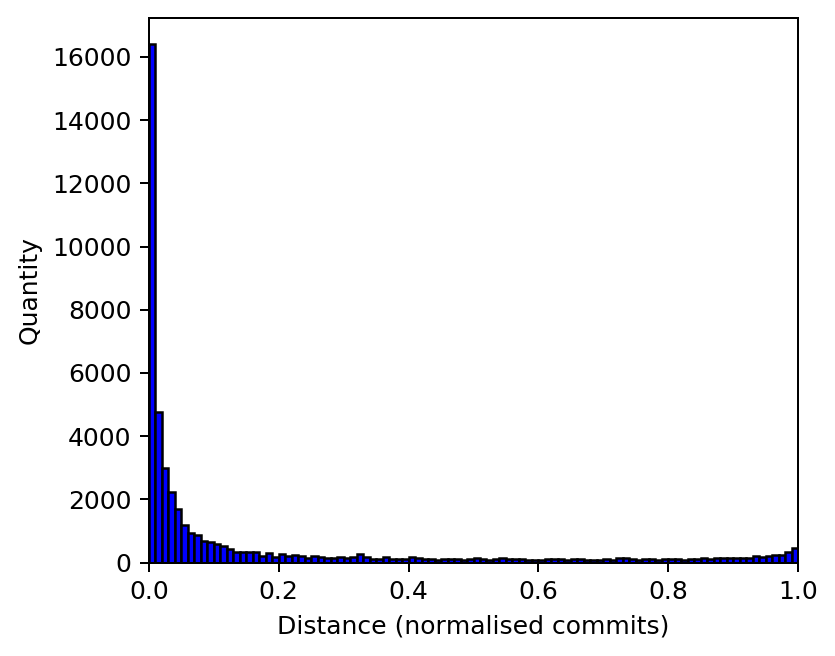
\includegraphics[width=\columnwidth]{graph000}%
\caption{\label{fig:c-commits}Normalised location of regression by commit in C projects measured by commit}
\end{figure}

We also note that the number of regressions also increases slightly as the next release approaches (\ie\/ as we get closer to the initial end point of the bisection analysis).

In performing our regression analysis, we want to try to take into account the broad characteristics of the curve, in choosing the function space to perform the regression over.

We therefore consider three different regression functions and compare the results between the three: cubic polynomial, cubic polynomial divided by $x$, and exponentiated cubic polynomial. These were chosen for their likelihood of capturing both the very rapid rise in values needed towards the start of the function, and the slight rise in values towards the end of the function.

Each of these has three coefficients, $a_0$, $a_1$ and $a_2$, and can be represented equations as equations \ref{eqn:poly}, \ref{eqn:negpow} and \ref{eqn:exp} respectively.
\begin{align}
y &= a_2 x^2 + a_1 x + a_0 \label{eqn:poly} \\
y &= a_2 x + a_1 + a_0 x^{-1} \label{eqn:negpow} \\
y &= \e{a_2 x^2 + a_1 x + a_0} \label{eqn:exp}
\end{align}

In order to establish which is the most accurate we perform regression analysis on the data using each of the three equation types. We then calculate the regression error to establish which provides the best fit.

\subsection{Distance metric}

We also consider that {\it commits\/} may not be the best feature to use when measuring the distance between release, regression and fix. We therefore also apply our regression analysis to two other features which we determine from the git commit data extracted from GitHub.

\begin{figure}[t]
\centering
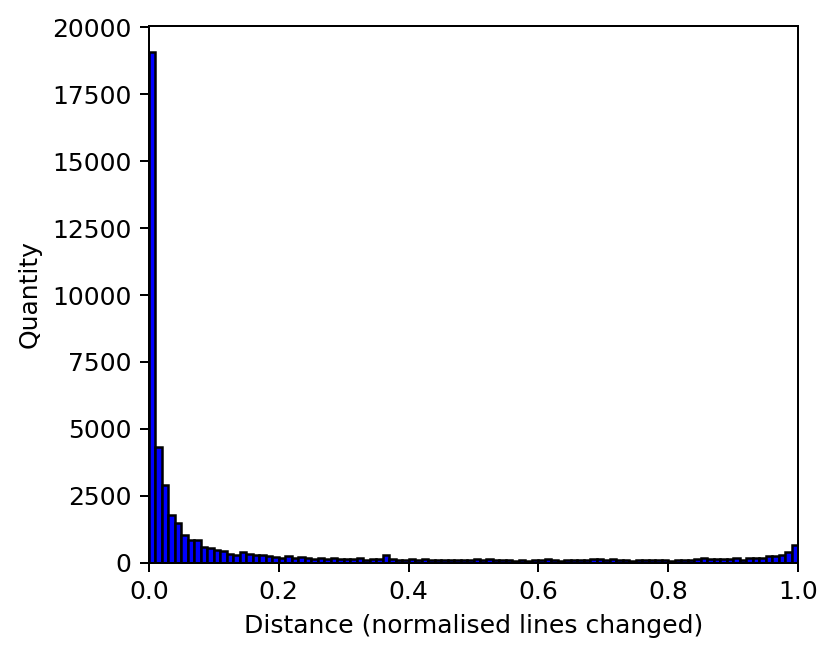
\includegraphics[width=\columnwidth]{graph001}%
\caption{\label{fig:c-lines}Normalised location of regression by commit in C projects measured by lines changed}
\end{figure}

Figure \ref{fig:c-lines} shows the frequency data where distance is measured by {\it lines of code changed}, rather than number of commits. This is the most fine-grained measure that we consider. The information is extracted from the diff of the change. As with commits, we normalise the distances to lie between zero and one.

\begin{figure}[t]
\centering
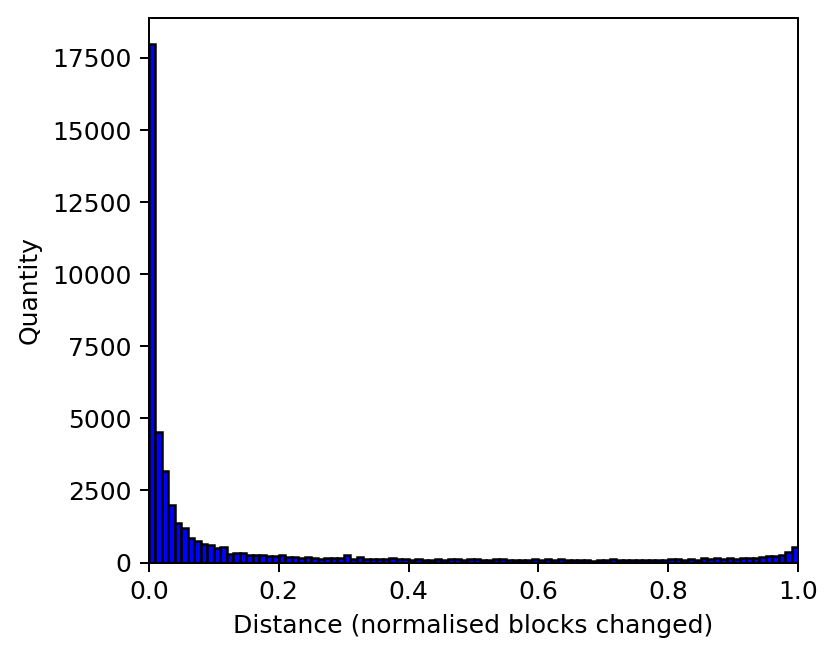
\includegraphics[width=\columnwidth]{graph002}%
\caption{\label{fig:c-blocks}Normalised location of regression by commit in C projects measured by hunks}
\end{figure}

Figure \ref{fig:c-blocks} shows similar frequency data using {\it hunks of code changed\footnote{A {\it hunk\/} of code is a series of lines where the code has been changed, surrounded by lines that have not changed, see for example \url{http://www.gnu.org/software/diffutils/manual/html_node/Hunks.html}}}. Again, this data is extracted from the git diff. Git uses a heuristic to distinguish between code hunks, which is largely aimed at improving the aesthetics and readability of a commit diff\footnote{See \url{https://github.com/git/git/commit/433860f3d0beb0c6f2}}.

We perform the same process on each of these metrics, collecting the data for all regressions, partitioning the results into buckets and performing similar regression analyses. For each of the three regression types we provide and compare the results for each of these three distance metrics.

\begin{figure}[t]
\centering
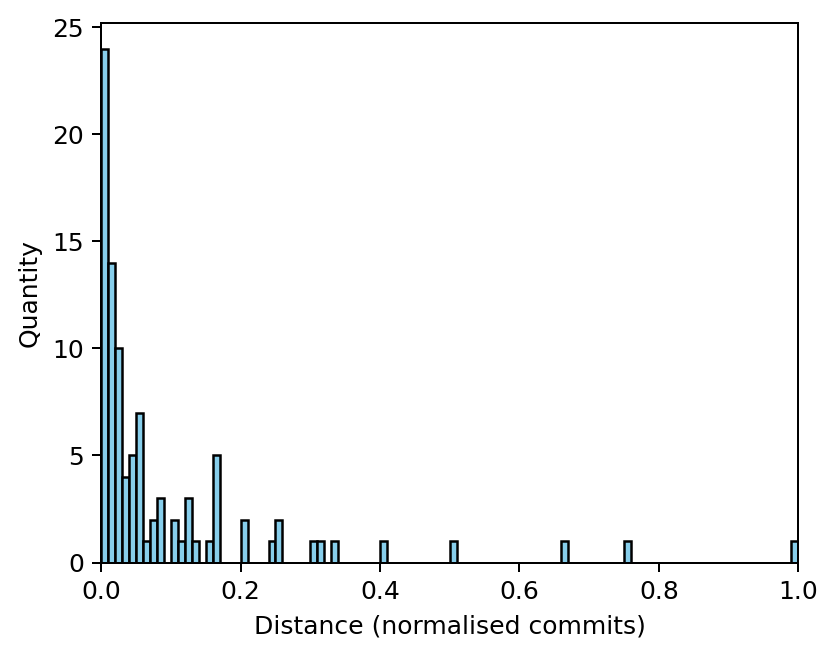
\includegraphics[width=\columnwidth]{graph010}%
\caption{\label{fig:javascript-commits}Normalised location of regression by commit in Javascript projects measured by commit}
\end{figure}

\begin{figure}[t]
\centering
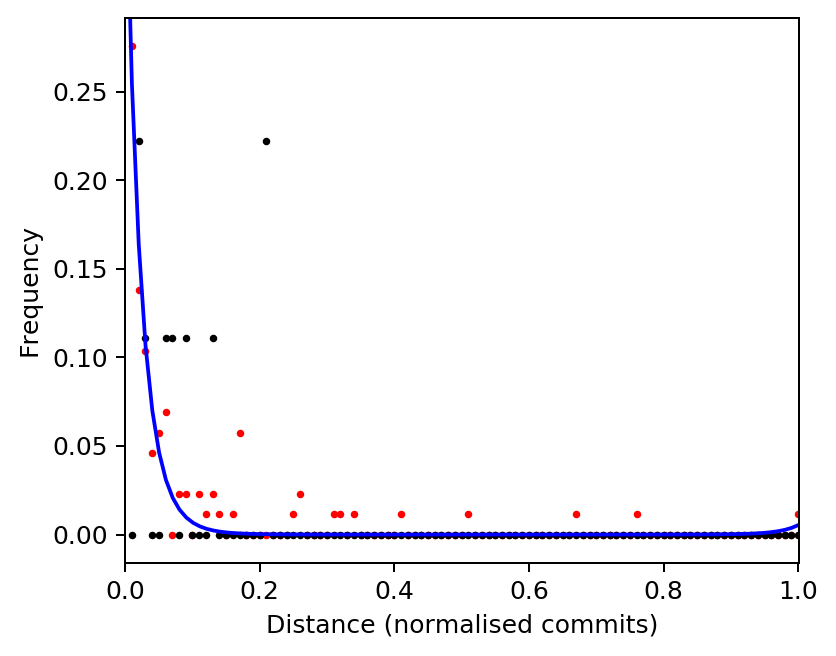
\includegraphics[width=\columnwidth]{graph011}%
\caption{\label{fig:javascript-lines}Normalised location of regression by commit in Javascript projects measured by lines changed}
\end{figure}

\begin{figure}[t]
\centering
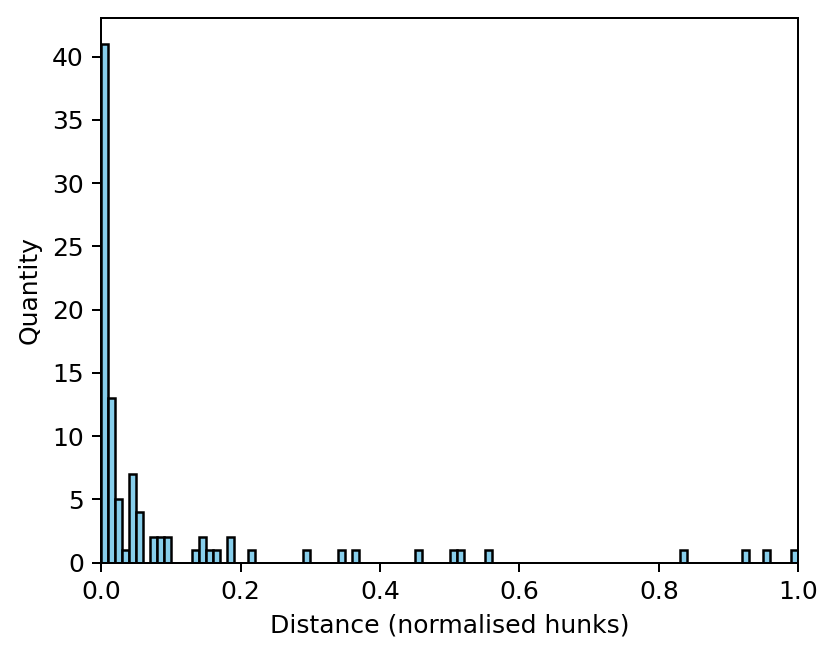
\includegraphics[width=\columnwidth]{graph012}%
\caption{\label{fig:javascript-blocks}Normalised location of regression by commit in Javascript projects measured by blocks changed}
\end{figure}

Figures \ref{fig:c-commits}--\ref{fig:c-blocks} show the frequency data collected for all C language projects on GitHub. For comparison, figures \ref{fig:javascript-commits}--\ref{fig:javascript-blocks} show the frequency data for the respective distance metrics for all Javascript language projects on GitHub. Apart from being a smaller population (587 C projects compared with 46 Javascript projects), Javascript is also a very different language to C, makes it an interesting comparison.

\subsection{Cubic polynomial regression}

For the cubic polynomial we use the standard matrix-based polynomial regression, which involves solving the following matrix equation for the polynomial coefficients $a_0, a_1$ and $a_2$.

\begin{equation}
\begin{bmatrix}
n          & \sum x_i   & \sum x_i^2 \\
\sum x_i   & \sum x_i^2 & \sum x_i^3 \\
\sum x_i^2 & \sum x_i^3 & \sum x_i^4 \\
\end{bmatrix}
\begin{bmatrix}
a_0 \\
a_1 \\
a_2 \\
\end{bmatrix}
=
\begin{bmatrix}
\sum y_i \phantom{x_i} \\
\sum x_i y_i           \\
\sum x_i^2 y_i         \\
\end{bmatrix}.
\end{equation}

In this equation $n$ is the number of buckets, the $x_i$ represent the normalised number of commits between 0 and 1, and the $y_i$ are the corresponding number of regressions in each bucket.

We can then replace the coefficients into Equation \ref{eqn:poly} in order to match the frequency distribution curve of the coding regressions.

\begin{figure}[t]
\centering
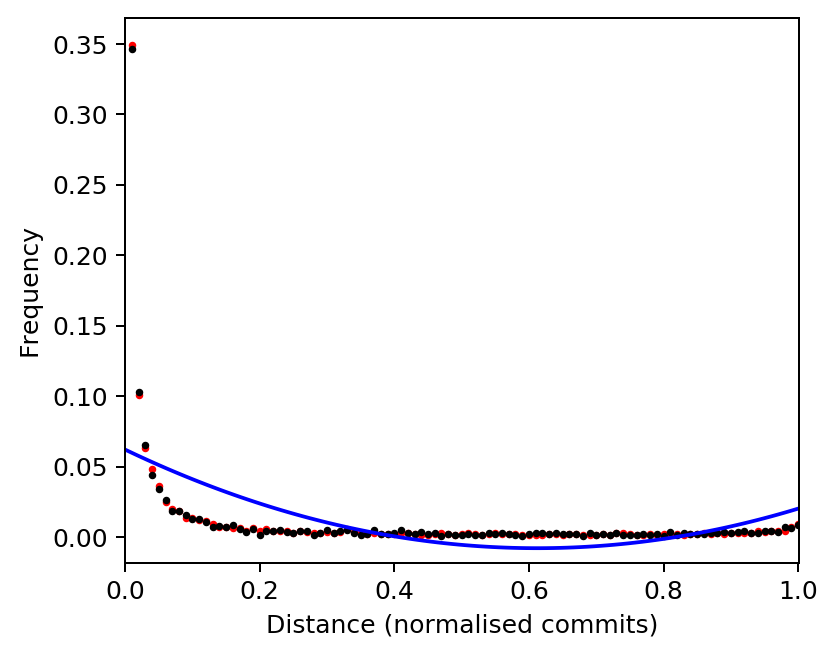
\includegraphics[width=\columnwidth]{graph003}%
\caption{\label{fig:c-linear}Linear regression applied to normalised commits for C programmes. Red dots represent learning data, black dots validation data, showing once instance taken from a 10-fold cross validation process. The line formula is $0.187x^{2} - 0.228x + 0.0622$.}
\end{figure}

The result of this for the C language data can be seen in Figure \ref{fig:c-linear}. The regression calculation returns the following coefficients:

\begin{align*}
a_1 & = 0.0622, \\
a_2 & = -0.228, \\
a_3 & = 0.187,
\end{align*}
giving a final cubic polynomial of $0.187x^{2} - 0.228x + 0.0622$ shown as the line in the graph. The dots in the graph represent the frequencies based on the data (\ie\/ the same data shown in Figure \ref{fig:c-commits} but scaled to represent probabilities). As we can see, a third-degree polynomial doesn't offer a fantastic fit to the data, and as such we decided to look at a number of other possible regression functions. We consider two of these in greater detail in the following sub sections.

\begin{figure}[t]
\centering
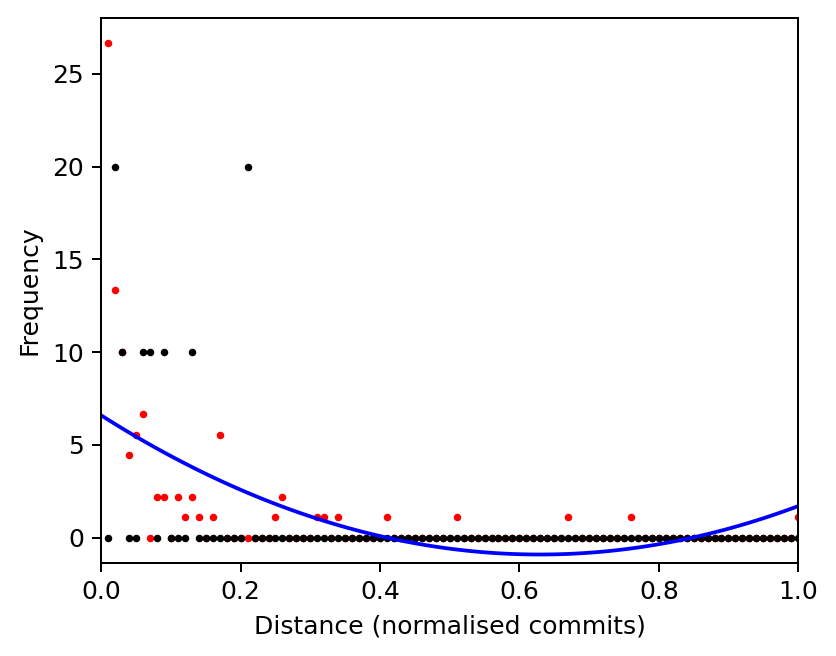
\includegraphics[width=\columnwidth]{graph013}%
\caption{\label{fig:javascript-linear}Linear regression applied to normalised commits for Javascript projects. Red dots represent learning data, black dots validation data, showing once instance taken from a 10-fold cross validation process. The line formula is $0.196x^{2} - 0.246x + 0.0682$.}
\end{figure}


For comparison, we also show the result of applying a linear regression to the Javascript data in Figure \ref{fig:javascript-linear}.

\subsection{Polynomial with negative power regression}

For the polynomial divided by $x$ (\ie\/ including a single negative power) we use the following matrix-based polynomial regression, solved with the least-square method, in order to calculate the coefficients $a_0, a_1$ and $a_2$.

\begin{equation}
\begin{bmatrix}
\sum x_i^{-2} & \sum x_i^{-1}        & n            \\
\sum x_i^{-1} & n                    & \sum x_i     \\
n             & \sum x_i \phantom{-} & \sum x_i^{2} \\
\end{bmatrix}
\begin{bmatrix}
a_0 \\
a_1 \\
a_2 \\
\end{bmatrix}
=
\begin{bmatrix}
\sum x_i^{-1} y_i        \\
\sum y_i \phantom{x_i -} \\
\sum x_i y_i \phantom{-} \\
\end{bmatrix}.
\end{equation}

In this equation $n$ is again the number of buckets, the $x_i$ represent the normalised number of commits between 0 and 1, and the $y_i$ are the corresponding number of regressions in each bucket.

We can then replace the coefficients into Equation \ref{eqn:negpow} in order to match the frequency distribution curve of the coding regressions.

\begin{figure}[t]
\centering
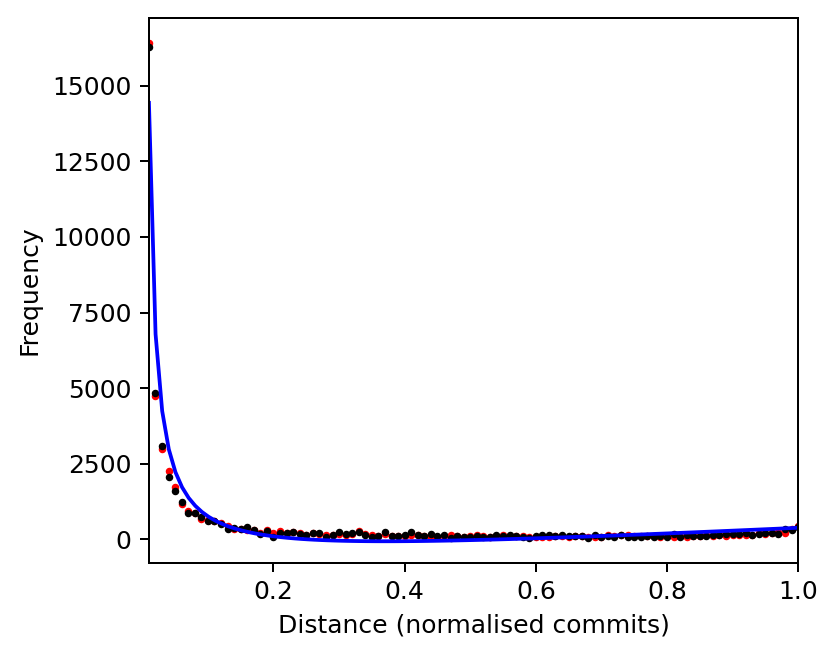
\includegraphics[width=\columnwidth]{graph004}%
\caption{\label{fig:c-negpow}Negative power regression applied to normalised commits for C programmes. Red dots represent learning data, black dots validation data, showing once instance taken from a 10-fold cross validation process. The line formula is $0.024x - 0.0192 + 0.00329x^{-1}$.}
\end{figure}

The result of this for the C language data can be seen in Figure \ref{fig:c-negpow}. In this case the calculated coefficients are as follows:

\begin{align*}
a_1 & = 0.00329, \\
a_2 & = -0.0192, \\
a_3 & = 0.024,
\end{align*}
giving a final negative-power polynomial of $0.024x - 0.0192 + 0.00329x^{-1}$ shown as the line in the graph. Here again the dots represent the frequencies based on the data scaled to represent probabilities. The fit here is visibly better than for the linear regression.

\begin{figure}[t]
\centering
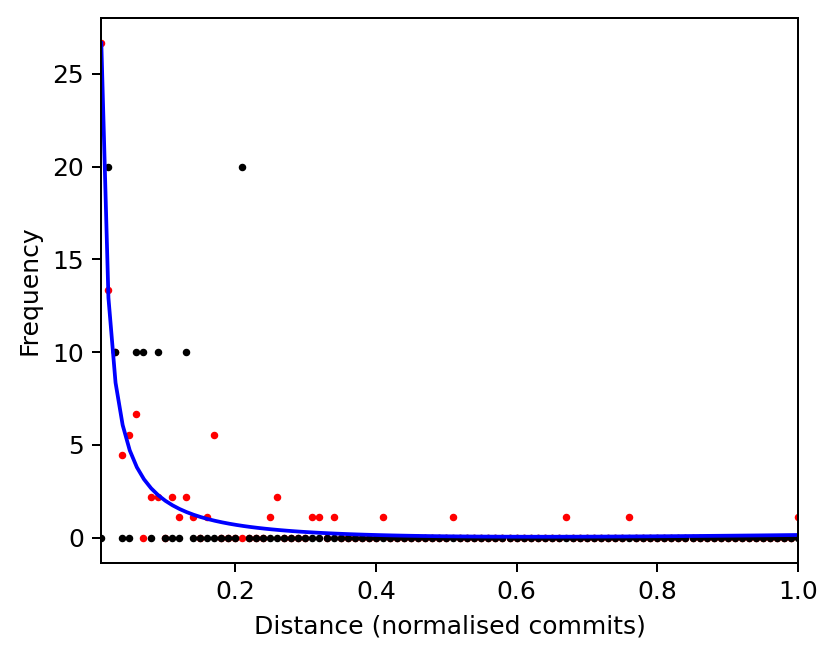
\includegraphics[width=\columnwidth]{graph014}%
\caption{\label{fig:javascript-negpow}Negative power regression applied to normalised commits for Javascript projects. Red dots represent learning data, black dots validation data, showing once instance taken from a 10-fold cross validation process. The line formula is $0.00719x - 0.00852 + 0.00287x^{-1}$.}
\end{figure}

For comparison, we also show the result of applying a linear regression to the Javascript data in Figure \ref{fig:javascript-negpower}.

\subsection{Exponentiated polynomial regression}

In the exponential case there is unfortunately no algebraic solution for finding the coefficients. Instead we apply the Newton-Raphson method to heuristically reduce the least-square error and converge on the optimal coefficients needed to approximate the coding regression distribution.

For points $(x_i, y_i)$ on the curve, and polynomial $p(x) = a_0 + a_1 x_i + a_2 x_i^2$, we want to minimise the error
$$
E = \sum_{0 \le i < n} \left( y_i - \e{p(x_i)} \right)^2 .
$$

The minimum value of $E$ will occur when the derivative is zero, hence we minimise the error by attempting to find $a_i$ such that the following partial derivatives are as close to zero as possible for $0 \le i < 2$:

$$
\partdiff{E}{a_j} = \sum_{0 \le i < n} \left( 2 x_i^j \e{2 p(x_i)} - 2 y_i x_i^j \e{p(x_i)} \right) .
$$

As mentioned, we're not able to solve this algebraically, so instead we use Newton-Raphson to find a numerical solution.


We start with an approximation of the coefficients by taking the logarithm of the $y$ values and applying a standard third-degree polynomial regression on them. This will exaggerate the effect of the errors as $x$ increases, but nevertheless provides a suitable set of initial values from which to apply Newton-Raphson.

We then take the partial derivative for each successive power, apply Newton-Raphson in order to find a new coefficient that reduces the error, and repeatedly cycle through the powers until the error falls below our chosen threshold. The second partical derivative is used for the Newton-Raphson refinement step.

$$
\partdiff[2]{E}{a_j} = \sum_{0 \le i < n} \left( 4 x_i^{2j} \e{2 p(x_i)} - 2 y_i x_i^{2j} \e{p(x_i)} \right) .
$$

\begin{figure}[t]
\centering
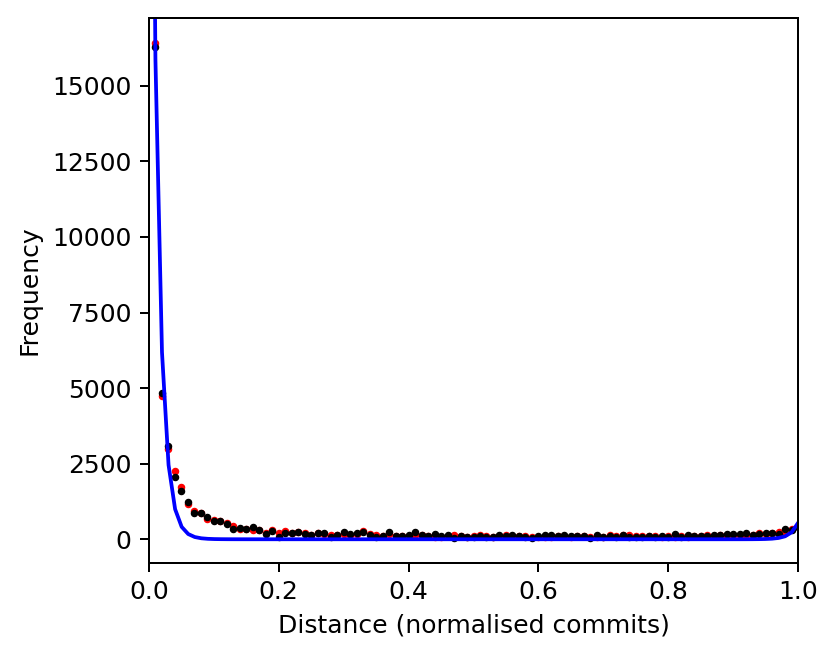
\includegraphics[width=\columnwidth]{graph005}%
\caption{\label{fig:c-exp}Exponentiated polynomial regression applied to normalised commits for C programmes. Red dots represent learning data, black dots validation data, showing once instance taken from a 10-fold cross validation process. The line formula is $e^{32.1x^{2} - 34.5x - 0.833}$.}
\end{figure}

\begin{figure}[t]
\centering
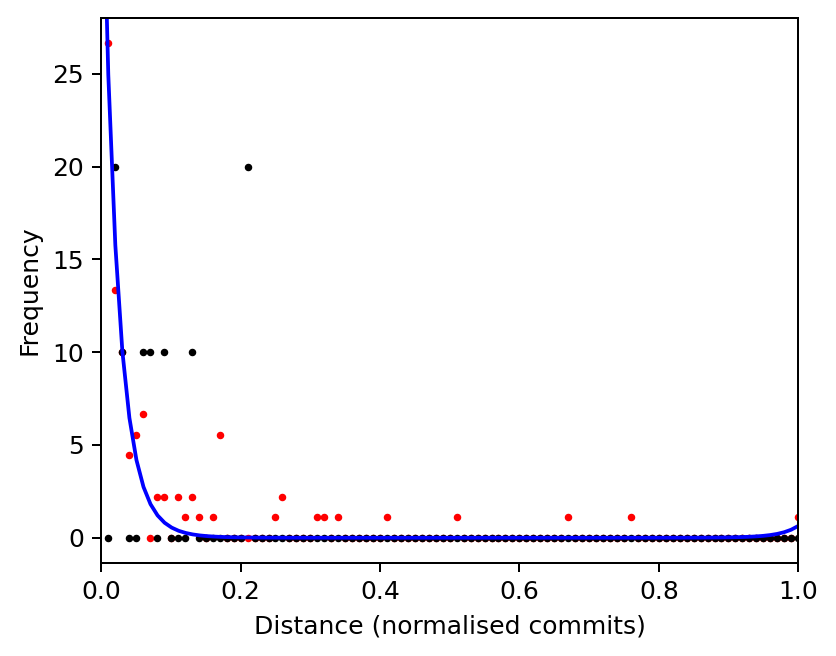
\includegraphics[width=\columnwidth]{graph015}%
\caption{\label{fig:javascript-exp}Exponentiated polynomial regression applied to normalised commits for Javascript projects. Red dots represent learning data, black dots validation data, showing once instance taken from a 10-fold cross validation process. The line formula is $e^{40.3x^{2} - 44.6x - 0.923}$.}
\end{figure}

The result of applying this approach for the C language data can be seen in Figure \ref{fig:c-exp} and for Python projects in Figure \ref{fig:javascript-exp}. In the case of C projects, the resulting coefficients are as follows:

\begin{align*}
a_1 & = -0.129, \\
a_2 & = -95.9, \\
a_3 & = 91.5,
\end{align*}
giving an equation of $e^{32.1x^{2} - 34.5x - 0.833}$, which is shown in the Figure \ref{fig:c-exp} as the solid line. The dots represent the frequencies based on the data scaled to represent probabilities. The fit here is again visibly better than for the linear regression.

\subsection{Experimental results}

We performed ther three different regression calculations on the data for all of the different languages collected, using each of the three distance measures: commits, lines and hunks. Each regression resulting in three coefficient values shown in Table \ref{table:coefficients}. The coefficients were calculated using regressions performed on the full set of data.

\begin{table*}[t!]
\begin{center}
\begin{tabular}{l | *{3}{d{3.4}} | *{3}{d{3.4}} | d{4.5} *{2}{d{3.4}} } \hline
  & \multicolumn{3}{c |}{Linear} & \multicolumn{3}{c |}{Negative power} & \multicolumn{3}{c}{Exponential} \\
  & \multicolumn{3}{c |}{$a_3 x^2 + a_2 + a_1$} & \multicolumn{3}{c |}{$a_3 x + a_2 + a_1 x^{-1}$} & \multicolumn{3}{c}{$\e{a_3 x^2 + a_2 x + a_1}$} \\
Category & \multicolumn{1}{c}{$a_3$} & \multicolumn{1}{c}{$a_2$} & \multicolumn{1}{c |}{$a_1$} & \multicolumn{1}{c}{$a_3$} & \multicolumn{1}{c}{$a_2$} & \multicolumn{1}{c |}{$a_1$} & \multicolumn{1}{c}{$a_3$} & \multicolumn{1}{c}{$a_2$} & \multicolumn{1}{c}{$a_1$} \\ \hline
C commits & 8774.8 & -10742.0 & 2926.2 & 1128.4 & -902.1 & 154.7 & 91.5 & -95.9 & 10.6 \\
C lines & 9274.2 & -11268.3 & 3023.1 & 1498.4 & -1193.6 & 174.9 & 120.2 & -124.7 & 11.1 \\
C hunks & 9081.1 & -11070.6 & 2988.5 & 1347.8 & -1076.5 & 167.0 & 105.9 & -110.4 & 10.9 \\ \hdashline
C++ commits & 738.9 & -917.8 & 249.7 & 118.7 & -101.2 & 14.9 & -1269.1 & -100.2 & 8.54 \\
C++ lines & 794.1 & -972.8 & 258.8 & 186.4 & -153.3 & 18.4 & -1075.8 & -189.7 & 9.68 \\
C++ hunks & 772.0 & -952.0 & 255.7 & 157.8 & -131.6 & 17.0 & -1052.6 & -149.7 & 9.18 \\ \hdashline
C\# commits & 170.9 & -212.4 & 58.2 & 28.6 & -23.9 & 3.52 & 26.1 & -139.7 & 7.37 \\
C\# lines & 186.3 & -228.6 & 61.2 & 43.5 & -35.6 & 4.32 & -411.9 & -205.4 & 8.33 \\
C\# hunks & 177.2 & -219.2 & 59.5 & 35.5 & -29.3 & 3.90 & -446.1 & -178.4 & 7.94 \\ \hdashline
Go commits & 9.70 & -12.0 & 3.31 & 0.534 & -0.488 & 0.142 & 11.1 & -24.2 & 2.50 \\
Go lines & 10.9 & -13.4 & 3.58 & 2.19 & -1.80 & 0.233 & 5.10 & -46.9 & 3.40 \\
Go hunks & 9.79 & -12.2 & 3.36 & 0.907 & -0.793 & 0.165 & 11.5 & -34.2 & 2.85 \\ \hdashline
Java commits & 2349.5 & -2892.0 & 770.7 & 496.4 & -416.5 & 52.2 & -5770.4 & -22.0 & 9.50 \\
Java lines & 2460.1 & -3005.8 & 790.8 & 594.5 & -492.8 & 57.4 & 210.0 & -229.2 & 11.1 \\
Java hunks & 2396.8 & -2940.1 & 779.0 & 538.6 & -449.1 & 54.4 & -6607.2 & -13.8 & 9.55 \\
JavaScript commits & 18.5 & -23.4 & 6.50 & 0.318 & -0.532 & 0.257 & 7.97 & -37.1 & 3.47 \\
JavaScript lines & 22.6 & -27.5 & 7.21 & 5.60 & -4.62 & 0.53 & 9.08 & -139.0 & 5.48 \\
JavaScript hunks & 20.6 & -25.4 & 6.82 & 2.87 & -2.49 & 0.385 & 19.6 & -69.4 & 4.30 \\ \hdashline
Objective-C commits & 18.6 & -24.0 & 7.24 & -0.561 & 0.498 & 0.236 & -5.27 & -27.0 & 3.26 \\
Objective-C lines & 25.4 & -31.3 & 8.63 & 4.72 & -3.70 & 0.531 & 8.69 & -137.1 & 5.46 \\
Objective-C hunks & 22.1 & -27.7 & 7.95 & 1.47 & -1.13 & 0.352 & 7.04 & -54.7 & 4.06 \\ \hdashline
Perl commits & 19.7 & -24.8 & 6.78 & 2.69 & -2.41 & 0.387 & 21.4 & -74.0 & 4.38 \\
Perl lines & 20.0 & -25.0 & 6.79 & 3.30 & -2.86 & 0.414 & 21.9 & -82.6 & 4.56 \\
Perl hunks & 19.7 & -24.6 & 6.73 & 3.16 & -2.76 & 0.407 & 24.7 & -81.5 & 4.53 \\ \hdashline
PHP commits & 81.2 & -100.5 & 26.9 & 13.8 & -12.0 & 1.66 & 6.98 & -143.0 & 6.64 \\
PHP lines & 85.8 & -105.2 & 27.8 & 18.1 & -15.3 & 1.88 & 33.3 & -149.4 & 6.84 \\
PHP hunks & 83.8 & -103.2 & 27.4 & 15.5 & -13.3 & 1.75 & 37.8 & -136.1 & 6.62 \\ \hdashline
Python commits & 210.8 & -260.2 & 68.9 & 40.6 & -35.1 & 4.52 & 26.7 & -169.5 & 7.93 \\
Python lines & 221.6 & -271.3 & 70.9 & 56.4 & -47.4 & 5.35 & 44.1 & -234.3 & 8.78 \\
Python hunks & 217.3 & -267.1 & 70.2 & 46.2 & -39.5 & 4.83 & 48.3 & -164.5 & 7.94 \\ \hdashline
R commits & 18.7 & -21.6 & 6.35 & 1.83 & -0.351 & 0.233 & 7.67 & -31.8 & 3.25 \\
R lines & 21.6 & -24.5 & 6.85 & 3.92 & -1.96 & 0.341 & 10.4 & -55.6 & 3.97 \\
R hunks & 19.1 & -22.1 & 6.45 & 2.29 & -0.714 & 0.258 & 8.24 & -40.7 & 3.51 \\ \hdashline
Ruby commits & 13.3 & -16.9 & 4.76 & 1.02 & -0.944 & 0.228 & 7.71 & -35.2 & 3.27 \\
Ruby lines & 14.5 & -18.1 & 5.01 & 2.72 & -2.29 & 0.321 & 19.9 & -55.1 & 3.87 \\
Ruby hunks & 12.4 & -15.9 & 4.57 & 1.77 & -1.51 & 0.263 & 16.7 & -45.9 & 3.55 \\ \hdashline
Rust commits & 31.0 & -38.9 & 11.0 & 3.97 & -3.29 & 0.598 & 17.8 & -105.6 & 5.22 \\
Rust lines & 34.4 & -42.8 & 11.8 & 7.63 & -6.21 & 0.805 & 15.5 & -188.3 & 6.42 \\
Rust hunks & 31.7 & -39.8 & 11.2 & 5.47 & -4.48 & 0.683 & -4.65 & -139.1 & 5.73 \\ \hdashline
Swift commits & 8.27 & -10.2 & 2.99 & -0.541 & 0.58 & 0.0662 & -11.4 & -9.83 & 1.71 \\
Swift lines & 9.28 & -11.4 & 3.29 & 1.85 & -1.33 & 0.202 & -4.34 & -39.7 & 3.14 \\
Swift hunks & 8.84 & -11.0 & 3.22 & 0.733 & -0.474 & 0.145 & 0.6 & -24.2 & 2.52
\end{tabular}
\caption{\label{table:coefficients}Regression coefficients.}
\end{center}
\end{table*}

In order to test Hypothesis \ref{hyp:algorithm} we need a means of comparing the goodness of fit of the different regression results. We do this by considering $E$ the {\it Root Mean Square Error\/}\footnote{See \url{https://en.wikipedia.org/w/index.php?title=Root-mean-square_deviation&oldid=1093261496}} and $R^"$ the {\it Coefficient of Determination\/}\footnote{See \url{https://en.wikipedia.org/w/index.php?title=Coefficient_of_determination&oldid=1096140789}}. If $(x_i, y_i)$ are the data points for $1 \le i \le n$ and $f : \mathbb{R} \mapsto \mathbb{R}$ is the function determined by performing the regression, then:

\begin{align}
E   & = \sqrt{\frac{\sum_i (y_i - f(x_i))^2}{n}}, \\
R^2 & = 1 - \frac{\sum_i (y_i - f(x_i))^2}{\sum_i (y_i - \bar{y})^2},
\end{align}
where $\bar{y}$ represents the arithmetical mean of the $y_i$. The Root Mean Square Error provides a measure for the error between the actual values and the predicted values (the regression function), meaning that the closer the value is to zero the better. The Coefficient of Determination is the proportion of the variation of the $y_i$ that is predictable from the $x_i$ using $f$. Hence values closer to one are better.

\begin{table*}[t!]
\begin{center}
\begin{tabular}{l | l l | l l | l l } \hline
  & \multicolumn{2}{c |}{Linear} & \multicolumn{2}{c |}{Negative power} & \multicolumn{2}{c}{Exponential} \\
Category & \multicolumn{1}{c}{$E$} & \multicolumn{1}{c |}{$R^2$} & \multicolumn{1}{c}{$E$} & \multicolumn{1}{c |}{$R^2$} & \multicolumn{1}{c}{$E$} & \multicolumn{1}{c}{$R^2$} \\ \hline
C commits & 1489.6 & 0.992455 & 360.1 & 0.999559 & 350.4 & 0.999581 \\
C lines & 1741.7 & 0.992043 & 543.7 & 0.999224 & {\bf 344.7} & {\bf 0.999688} \\
C hunks & 1638.8 & 0.992202 & 460.3 & 0.999385 & 348.6 & 0.999647 \\ \hdashline
C++ commits & 152.6 & 0.991908 & 53.96 & 0.998987 & 30.65 & 0.999668 \\
C++ lines & 200.9 & 0.991282 & 91.63 & 0.998187 & {\bf 25.23} & {\bf 0.999859} \\
C++ hunks & 180.7 & 0.991506 & 75.41 & 0.99852 & 28.19 & 0.999789 \\ \hdashline
C\# commits & 36.76 & 0.991794 & 14.98 & 0.998635 & 10.15 & 0.999361 \\
C\# lines & 47.63 & 0.991273 & 22.99 & 0.997974 & {\bf 9.949} & {\bf 0.999596} \\
C\# hunks & 41.99 & 0.991499 & 19.04 & 0.998254 & 10.28 & 0.999479 \\ \hdashline
Go commits & 2.546 & 0.991184 & 2.287 & 0.99214 & 2.366 & 0.991971 \\
Go lines & 3.151 & 0.990998 & 2.331 & {\bf 0.994286} & 2.488 & 0.993745 \\
Go hunks & 2.581 & 0.991276 & {\bf 2.207} & 0.992937 & 2.301 & 0.992664 \\ \hdashline
Java commits & 557.8 & 0.99146 & 234.4 & 0.99849 & 77.17 & 0.999836 \\
Java lines & 628.9 & 0.991245 & 287.9 & 0.998165 & 118.6 & {\bf 0.998907} \\
Java hunks & 588.0 & 0.99136 & 257.7 & 0.998341 & {\bf 69.94} & 0.999877 \\ \hdashline
JavaScript commits & 3.697 & 0.992084 & 3.137 & 0.993592 & 3.184 & 0.993524 \\
JavaScript lines & 6.041 & 0.991153 & 3.574 & 0.996422 & {\bf 2.766} & {\bf 0.997237} \\
JavaScript hunks & 4.467 & 0.991695 & 2.922 & 0.995887 & 2.941 & 0.995698 \\ \hdashline
Objective-C commits & 4.154 & 0.991832 & 3.697 & 0.993261 & 3.817 & 0.992788 \\
Objective-C lines & 6.390 & 0.991228 & 3.912 & 0.996434 & {\bf 3.345} & {\bf 0.997264} \\
Objective-C hunks & 4.805 & 0.99166 & 3.687 & 0.994685 & 3.784 & 0.994391 \\ \hdashline
Perl commits & 4.483 & 0.991752 & 2.633 & 0.997036 & {\bf 2.555} & {\bf 0.997132} \\
Perl lines & 4.855 & 0.991543 & 2.928 & 0.996677 & 2.732 & 0.99694 \\
Perl hunks & 4.828 & 0.991589 & 2.998 & 0.996588 & 2.889 & 0.996661 \\ \hdashline
PHP commits & 17.52 & 0.991789 & 7.694 & 0.998399 & {\bf 5.674} & 0.998988 \\
PHP lines & 20.14 & 0.991515 & 8.972 & 0.998327 & 5.933 & {\bf 0.99909} \\
PHP hunks & 18.69 & 0.991684 & 8.428 & 0.99828 & 6.333 & 0.998777 \\ \hdashline
Python commits & 47.70 & 0.991616 & 19.75 & 0.998563 & 10.09 & 0.999589 \\
Python lines & 59.10 & 0.991164 & 27.69 & 0.998059 & {\bf 6.836} & {\bf 0.999881} \\
Python hunks & 51.05 & 0.991476 & 20.72 & 0.998595 & 7.986 & 0.999782 \\ \hdashline
R commits & 4.468 & 0.990979 & {\bf 4.075} & 0.992125 & 4.315 & 0.991175 \\
R lines & 5.227 & 0.990865 & 4.306 & {\bf 0.993174} & 4.533 & 0.992428 \\
R hunks & 4.692 & 0.990895 & 4.226 & 0.991929 & 4.448 & 0.991069 \\ \hdashline
Ruby commits & 3.253 & 0.991552 & {\bf 2.536} & 0.994412 & 2.571 & 0.994321 \\
Ruby lines & 4.030 & 0.991224 & 2.743 & {\bf 0.995038} & 2.903 & 0.994592 \\
Ruby hunks & 3.531 & 0.991236 & 2.555 & 0.994688 & 2.676 & 0.994413 \\ \hdashline
Rust commits & 7.053 & 0.991643 & 4.324 & 0.996412 & 4.184 & 0.996325 \\
Rust lines & 9.266 & 0.991199 & 5.197 & 0.997001 & {\bf 3.733} & {\bf 0.998137} \\
Rust hunks & 7.877 & 0.99144 & 4.596 & 0.996233 & 4.015 & 0.996167 \\ \hdashline
Swift commits & 2.638 & 0.990723 & 2.647 & 0.990588 & 2.624 & 0.990747 \\
Swift lines & 3.167 & 0.990606 & 2.531 & {\bf 0.993124} & 2.670 & 0.992618 \\
Swift hunks & 2.781 & 0.990814 & {\bf 2.486} & 0.992168 & 2.588 & 0.99175
\end{tabular}
\caption{\label{table:regression}Average Standard Error and Residual values with 10-fold cross-validation. Lowest errors and highest residuals emphasised in bold.}
\end{center}
\end{table*}

Table \ref{table:regression} shows the values for $E$ and $R^2$ for each of the regressions performed. For each language the optimal results for $E$ and $R^2$ have been emphasised in bold. These values are mean values averaged across the ten cross-validation experiments.

In the largest number of cases (7 out of 14) the exponential regression applied using lines changed as the distance metric gave the lowest Root Mean Square Error and the highest Coefficient of Determination. In the case of Perl the exponential regression applied to commits gave the best fit. In the remaining cases the restults showed a lack of consistency between the Root Mean Square Error and Coefficient of Determination. The reasons for this are unclear, but can potentially be put down to the smaller datasets for many of the languages (see Table \ref{table:project-stats}) with the potential to introduce noise.

In the next section we will apply the results in order to develop an optimised bisect algorithm, and measure its effectiveness.

\section{Application}

Having refuted the claim that regressions are uniformly distributed, and established that a distance measure based on lines-changed modelled using an exponentiated polynomial provide the best fit for the data amongst the options tested, we now turn to applying these results to the bisect algorithm itself.

Our approach involves using the frequency distribution modelled by our function in order to transform the frequency space, as far as possible, into a uniform distribution. We then apply the original bisect algorithm to this transformed distribution.

In order to transoform the frequency distrubition we weight the distances based on the modelled function.

If $C_1, C_2 \in [0, 1]$ are points on the normalised interval between $A$ and $B$, then we set the distance metric $d : [0, 1] \times [ 0, 1 ] \to [ 0, 1 ]$ to be:
$$
d(C_1, C_2) = \int_{C_1}^{C_2} f(x) \ {\rm d}x .
$$

Since there's no algebraic solution we perform a numerical approximation, which will be more than good enough for our purposes since our distance metric is discrete (quantised by the number of lines in the code).

We use the exponential polynomial with using the coefficients shown in table \ref{table:coefficients} as the distance metric for our bisect algorithm and apply it to all of the results collected from Github. For comparison we do this using all three of our metrics: commits, lines and hunks. Finally we also do the same for the standard bisect algorithm (uniform distribution based on commits).

Table \ref{table:bisectsteps} summarises the results, showing the mean and standard deviation of the number of steps required to succesfully find the regression commit when using the various distance metrics. The values are calculated by reapplying our amended bisect algorithm to all of the projects on GitHub, catergories by language once again.

As we can see, in all cases the amended algorithm using a weighted distance metric provides a lower mean than the standard case. In other words, a weighted distance metric will find the regression commit in a fewer number of steps than just by using the standard bisect algorithm as employed by {\code git bisect}.

We provide a slightly more detailed breakdown this data for the C language in Figure \ref{fig:c-bisect}. The mean and standard deviation are marked on as the dashed and dotted lines respectively. This gives an idea of the distribution of number of steps needed across the C projects that had regression commits.

Figure \ref{fig:javascript-bisect} shows a similar breakdown of the results for the JavaScript language.

\begin{table*}[t!]
\begin{center}
\begin{tabular}{l | *{2}{d{3.3}} | *{2}{d{3.3}} | *{2}{d{3.3}} | *{2}{d{3.3}}} \hline
 & \multicolumn{2}{c |}{Commits} & \multicolumn{2}{c |}{Weighted commits} & \multicolumn{2}{c |}{Weighted lines} & \multicolumn{2}{c}{Weighted hunks} \\
Language & \multicolumn{1}{c}{$\mu$} & \multicolumn{1}{c |}{$\sigma$} & \multicolumn{1}{c}{$\mu$} & \multicolumn{1}{c |}{$\sigma$} & \multicolumn{1}{c}{$\mu$} & \multicolumn{1}{c |}{$\sigma$} & \multicolumn{1}{c}{$\mu$} & \multicolumn{1}{c}{$\sigma$} \\ \hline
C & 13.20 & 4.29 & 12.6 & 6.52 & 12.9 & 6.58 & 12.8 & 6.57 \\
C++ & 7.71 & 3.17 & 4.85 & 3.77 & 5.21 & 3.85 & 4.98 & 3.8 \\
C\# & 7.91 & 4.17 & 4.8 & 3.43 & 5.01 & 3.61 & 4.87 & 3.41 \\
Go & 5.02 & 2.26 & 3.77 & 1.85 & 3.77 & 2.02 & 3.73 & 1.71 \\
Java & 11.2 & 3.93 & 8.4 & 5.24 & 8.49 & 5.44 & 8.47 & 5.2 \\
JavaScript & 5.15 & 2.56 & 3.2 & 1.54 & 3.17 & 1.68 & 3.23 & 1.67 \\
Objective-C & 4.07 & 2.56 & 2.73 & 1.53 & 2.65 & 1.73 & 2.71 & 1.61 \\
Perl & 6.07 & 2.81 & 3.47 & 1.67 & 3.81 & 1.79 & 3.62 & 1.72 \\
PHP & 9.68 & 3.28 & 6.53 & 3.49 & 6.65 & 3.38 & 6.44 & 3.3 \\
Python & 8.96 & 3.47 & 4.94 & 3.46 & 5.44 & 3.44 & 5.09 & 3.27 \\
R & 6.61 & 2.7 & 6.2 & 3.23 & 6.3 & 3.39 & 6.07 & 3.11 \\
Ruby & 5.35 & 2.74 & 3.49 & 1.84 & 3.53 & 1.87 & 3.49 & 1.79 \\
Rust & 7.66 & 2.78 & 5.73 & 3.4 & 5.9 & 3.86 & 5.9 & 3.45 \\
Swift & 3.6 & 2.38 & 3.09 & 1.97 & 2.75 & 1.99 & 2.97 & 2.08 \\
\end{tabular}
\caption{\label{table:bisectsteps}Average number of bisect steps required to identify the regression commit.}
\end{center}
\end{table*}


\begin{figure*}[t]
\centering
\subfloat[]{
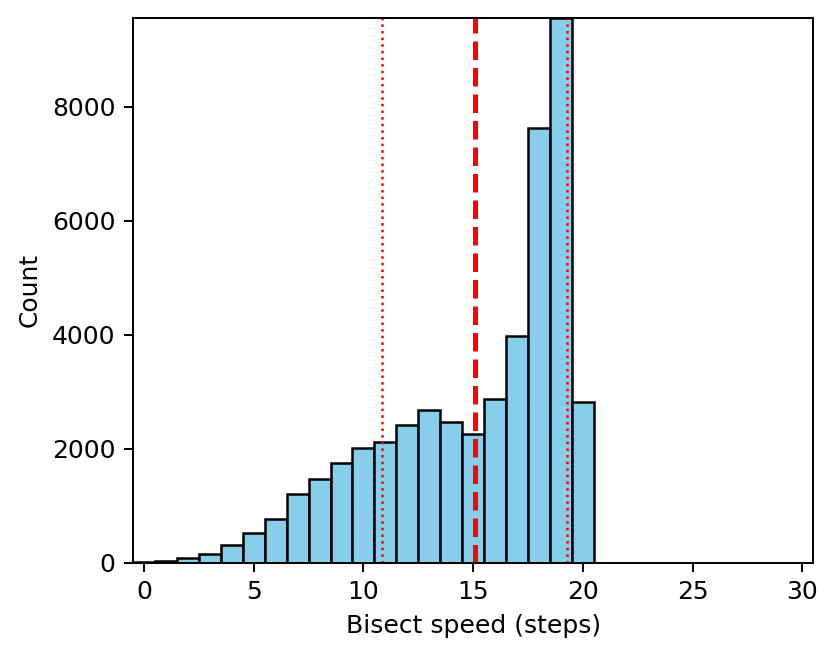
\includegraphics[width=\columnwidth]{graph006}%
\label{fig:c-bisect-commits}}
\hfil
\subfloat[]{
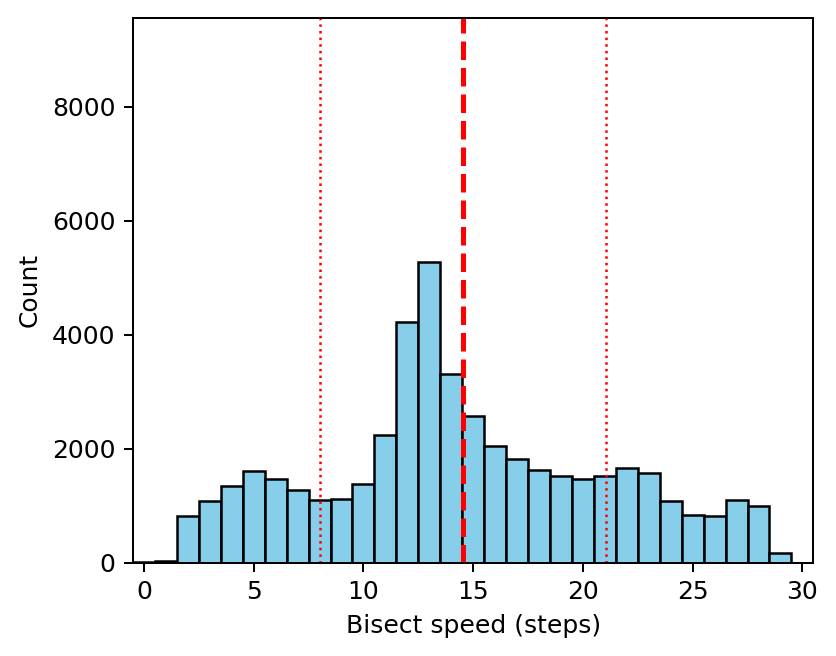
\includegraphics[width=\columnwidth]{graph007}%
\label{fig:c-bisect-commits-weighted}}
\hfil
\subfloat[]{
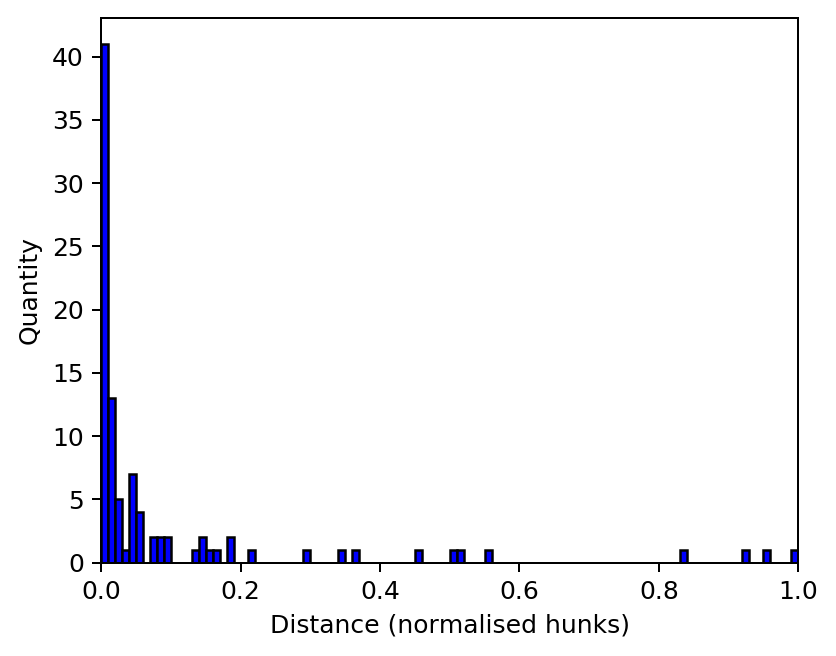
\includegraphics[width=\columnwidth]{graph008}%
\label{fig:c-bisect-lines-weighted}}
\hfil
\subfloat[]{
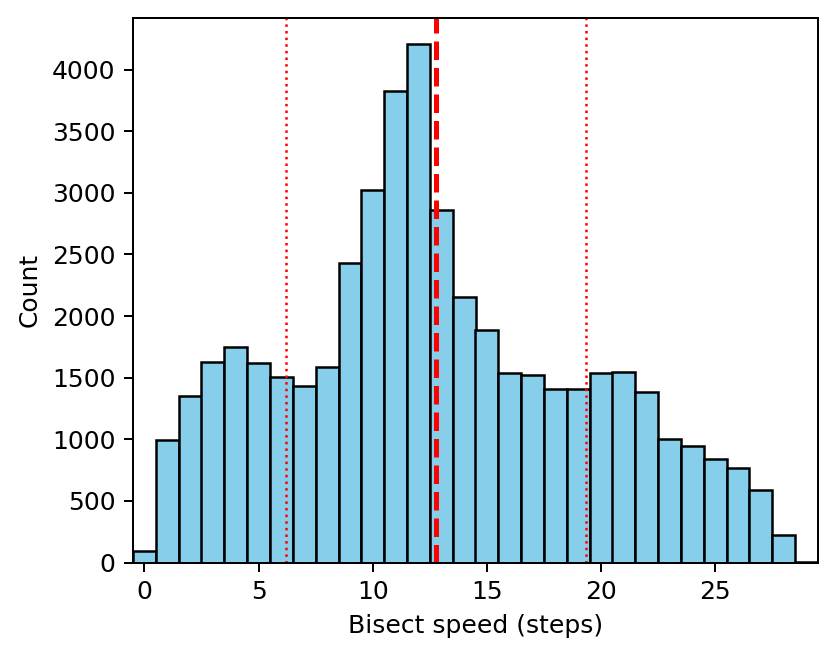
\includegraphics[width=\columnwidth]{graph009}%
\label{fig:c-bisect-hunks-weighted}}
\caption{\label{fig:c-bisect}Histograms for the C language of the number of steps required to complete the bisect algorithm using (a) the standard metrix; (b) the weighted commit metric; (c) the weighted lines changed metric; (d) the weighted hunks changed metric. The dashed line indicates the mean, the dotted lines a one-standard-deviation interval on each side it.}
\end{figure*}

\begin{figure*}[t]
\centering
\subfloat[]{
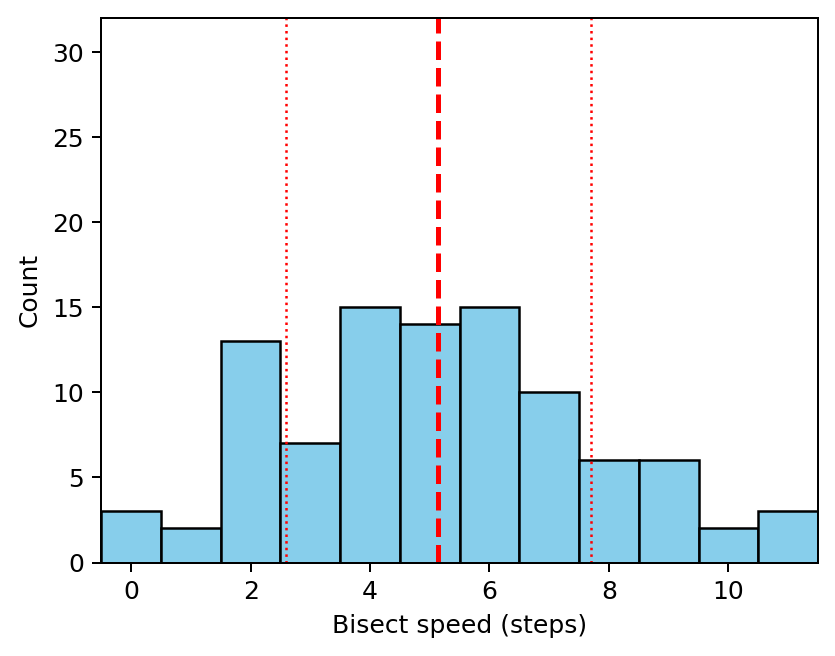
\includegraphics[width=\columnwidth]{graph016}%
\label{fig:javascript-bisect-commits}}
\hfil
\subfloat[]{
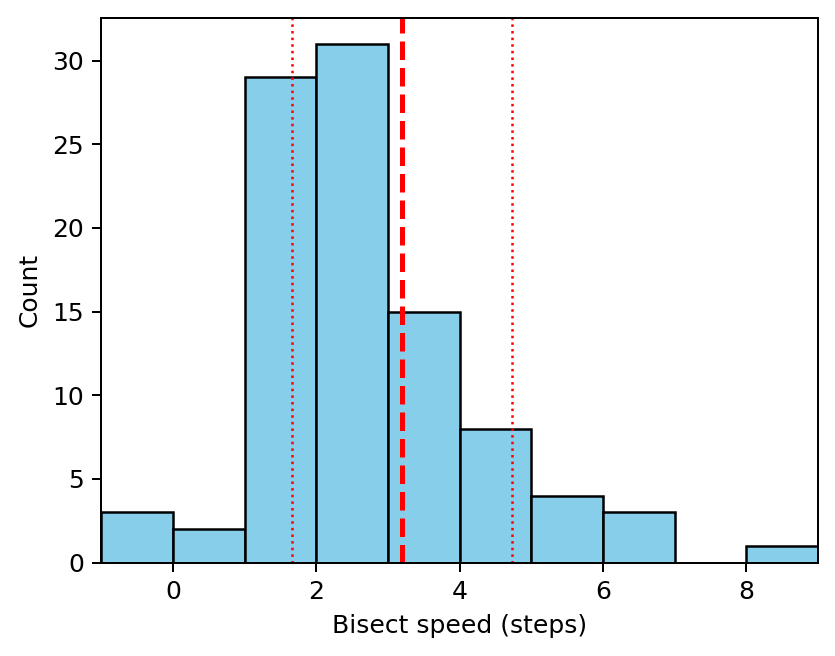
\includegraphics[width=\columnwidth]{graph017}%
\label{fig:javascript-bisect-commits-weighted}}
\hfil
\subfloat[]{
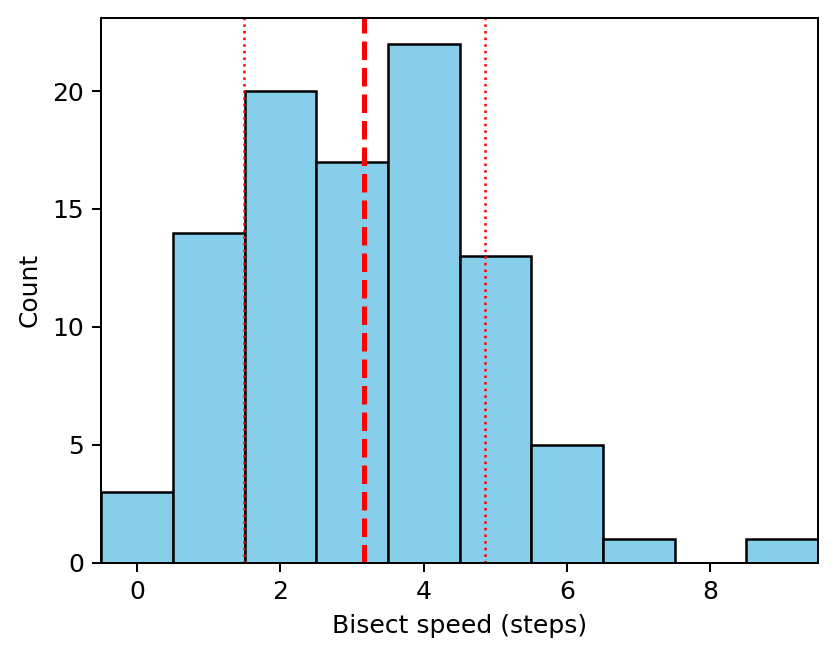
\includegraphics[width=\columnwidth]{graph018}%
\label{fig:javascript-bisect-lines-weighted}}
\hfil
\subfloat[]{
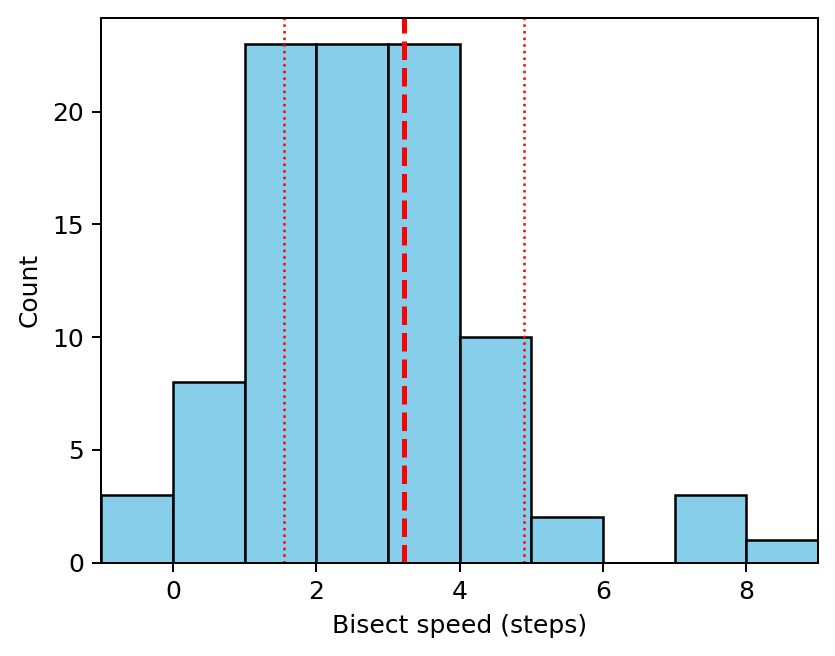
\includegraphics[width=\columnwidth]{graph019}%
\label{fig:javascript-bisect-hunks-weighted}}
\caption{\label{fig:javascript-bisect}Histograms for the JavaScript language of the number of steps required to complete the bisect algorithm using (a) the standard metrix; (b) the weighted commit metric; (c) the weighted lines changed metric; (d) the weighted hunks changed metric. The dashed line indicates the mean, the dotted lines a one-standard-deviation interval on each side it.}
\end{figure*}



\section{Limitations}

See \cite{moser2008} for examples.


\section{Related work}

Many of the areas that this work relates to are heavily researched with a broad body of literature to consider. The use of tests to determine regressions \cite{} and the general area of defect prediction and bug localisation \cite{kamei2013, shimagaki2016, yan2019}. Metrics for defect prediction range from the number of files or lines-of-code changed \cite{moser2008}, to the time of day a commit was made \cite{eyolfson2011}.

A portion of this work has focussed especially on identifying defect-introducing or fix-inducing changes in source code. In order to identify the commits being reverted, and the versions for which the regression was identified, we follow the approach of Shimagaki \etal \cite{shimagaki2016}. The SZZ algorithm \cite{sliwerski2005} is often used to detect bugs in code contained in a version control system. This approach doesn't fit with our requirements, since we're particularly interested in fix-inducing changes associated with regressions that lead to reverts. Moreover the SZZ approach requires correlation with bug tracking information, which we don't have access to for all of the projects hosted on GitHub.

Another important area that stems from this is in correlating fix-inducing code with other factors. This is often motivated as a means to predict the likelihood that any particular commit is likely to introduce a fix-inducing bug. This has direct relevance to our work, since these same characteristics are potential inputs for our algorithm. Yan \etal \cite{yan2019} identify lines added, lines deleted, developer experience, number of developers and number of unique commits to a file are the most discriminative features in identifying reverted commits.

A notable feature of these studies is that they tend to focus on small collections of often large software projects. For example, Moser \etal \cite{moser2008} consider three different Eclipse releases; Kamei \etal \cite{kamei2013} consider six open source projects and five commercial (closed-source) projects; Shimagaki \etal \cite{shimagaki2016} consider four open source and two proprietary. Ziftci \etal \cite{ziftci2013, ziftci2017} are somewhat exceptional in considering 140 projects internal to Google. We take this a stage further by considering all XXXXXX of the publicly available projects on GitHub. While not all of these have overt revert commits, the XXX projects with such commits is a notable increase compared to these other studies.

However, despite its widespread use and venerable age (in software engineering terms) there are very few that have attempted to optimise {\code git bisect} directly.

One exception is the work of Saha and Gligoric who introduced the idea of Selective Bisection Debugging in 2017 \cite{saha2017}. this combines {\it test selection\/} with {\it commit selection\/} to reduce the number of bisection steps. Test selection involves the selection of specific tests from a test suite that relate to a regression (\ie\/ the tests that fail), while commit selection involves selecting only those commits which are likely to have an effect on the tests (\eg\/ using code coverage analysis).

The authors demonstrate significant advantages using the technique, with average time savings between 24\% and 60\% across 10 different open source projects, and using the ``all tests after failing tests'' approach in which only the tests failing due to the regression are re-run at each step, with a second step of running all the tests in case the subset passes.

The obvious downside of this approach compared to the approach we propose is that it relies on pre-defined test cases with good programme coverage in order to be effective, which may not be the case for all projects. On the other hand, our approach can be applied even for bugs that only permit a manual test process.

Recent work at Google by Ziftci and Reardon \cite{ziftci2017}, apparently extending earlier work presented by Ziftci and Ramavajjala as a Google TechTalk \cite{ziftci2013}, has looked at probabilistically identifying the most likely changesets (a concept similar to a commit) to have caused regressions when periodic automated testing of builds fails. The changelists between the successful test passing and the successful test failing are passed through a heuristic which assigns a ``suspiciousness'' value to them. This is based on the size of the change, and the depth of the change in the dependency graph. The priority list is then sent to developers so they can establish for certain which changelist caused the regression. 

The ultimate goal is similar to that of related work such as that of Kamei \etal, which is to focus review efforts in the code most likely to introduce (or to have introduced) defects. The focus of these studies is therefore a little different from ours, since none of these studies consider using the results as input to the bisection algorithm.

Indeed Ziftci \etal explicitly discount bisection as an approach since the time required to re-run tests in the cases they consider can be prohibitive. They leave it to the developers of different components to ultimately make a decision about which changelists to focus on.

Nevertheless a natural question that arises is whether the same suspiciousness heuristics or defect-prediction models could be applied to a bisection approach to speed up its operation. We believe this to be the case. 

\section{Discussion and Conclusions}

Reading: Dambros2010 page 6.


yan2019

X. Yang, D. Lo, X. Xia, Y. Zhang, and J. Sun, “Deep learning for just-in-time defect prediction,” in Software Quality, Reliability and Security (QRS), 2015 IEEE International Conference on, Aug 2015, pp. 17–26.

S. Kim, E. J. W. Jr., and Y. Zhang, “Classifying software changes: Clean or buggy?” IEEE Transactions on Software Engineering, vol. 34, no. 2, pp. 181–196, March 2008.

S. Kim, T. Zimmermann, K. Pan, and E. J. J. Whitehead, “Automatic identification of bug-introducing changes,” in Proceedings of the 21st IEEE/ACM International Conference on Automated Software Engineering, ser. ASE ’06. Washington, DC, USA: IEEE Computer Society, 2006, pp. 81–90.


 

% An example of a floating figure using the graphicx package.
% Note that \label must occur AFTER (or within) \caption.
% For figures, \caption should occur after the \includegraphics.
% Note that IEEEtran v1.7 and later has special internal code that
% is designed to preserve the operation of \label within \caption
% even when the captionsoff option is in effect. However, because
% of issues like this, it may be the safest practice to put all your
% \label just after \caption rather than within \caption{}.
%
% Reminder: the "draftcls" or "draftclsnofoot", not "draft", class
% option should be used if it is desired that the figures are to be
% displayed while in draft mode.
%
%\begin{figure}[!t]
%\centering
%\includegraphics[width=2.5in]{myfigure}
% where an .eps filename suffix will be assumed under latex, 
% and a .pdf suffix will be assumed for pdflatex; or what has been declared
% via \DeclareGraphicsExtensions.
%\caption{Simulation results for the network.}
%\label{fig_sim}
%\end{figure}

% Note that the IEEE typically puts floats only at the top, even when this
% results in a large percentage of a column being occupied by floats.
% However, the Computer Society has been known to put floats at the bottom.


% An example of a double column floating figure using two subfigures.
% (The subfig.sty package must be loaded for this to work.)
% The subfigure \label commands are set within each subfloat command,
% and the \label for the overall figure must come after \caption.
% \hfil is used as a separator to get equal spacing.
% Watch out that the combined width of all the subfigures on a 
% line do not exceed the text width or a line break will occur.
%
%\begin{figure*}[!t]
%\centering
%\subfloat[Case I]{\includegraphics[width=2.5in]{box}%
%\label{fig_first_case}}
%\hfil
%\subfloat[Case II]{\includegraphics[width=2.5in]{box}%
%\label{fig_second_case}}
%\caption{Simulation results for the network.}
%\label{fig_sim}
%\end{figure*}
%
% Note that often IEEE papers with subfigures do not employ subfigure
% captions (using the optional argument to \subfloat[]), but instead will
% reference/describe all of them (a), (b), etc., within the main caption.
% Be aware that for subfig.sty to generate the (a), (b), etc., subfigure
% labels, the optional argument to \subfloat must be present. If a
% subcaption is not desired, just leave its contents blank,
% e.g., \subfloat[].


% An example of a floating table. Note that, for IEEE style tables, the
% \caption command should come BEFORE the table and, given that table
% captions serve much like titles, are usually capitalized except for words
% such as a, an, and, as, at, but, by, for, in, nor, of, on, or, the, to
% and up, which are usually not capitalized unless they are the first or
% last word of the caption. Table text will default to \footnotesize as
% the IEEE normally uses this smaller font for tables.
% The \label must come after \caption as always.
%
%\begin{table}[!t]
%% increase table row spacing, adjust to taste
%\renewcommand{\arraystretch}{1.3}
% if using array.sty, it might be a good idea to tweak the value of
% \extrarowheight as needed to properly center the text within the cells
%\caption{An Example of a Table}
%\label{table_example}
%\centering
%% Some packages, such as MDW tools, offer better commands for making tables
%% than the plain LaTeX2e tabular which is used here.
%\begin{tabular}{|c||c|}
%\hline
%One & Two\\
%\hline
%Three & Four\\
%\hline
%\end{tabular}
%\end{table}


% Note that the IEEE does not put floats in the very first column
% - or typically anywhere on the first page for that matter. Also,
% in-text middle ("here") positioning is typically not used, but it
% is allowed and encouraged for Computer Society conferences (but
% not Computer Society journals). Most IEEE journals/conferences use
% top floats exclusively. 
% Note that, LaTeX2e, unlike IEEE journals/conferences, places
% footnotes above bottom floats. This can be corrected via the
% \fnbelowfloat command of the stfloats package.




\section{Conclusion}
The conclusion goes here.





% if have a single appendix:
%\appendix[Proof of the Zonklar Equations]
% or
%\appendix  % for no appendix heading
% do not use \section anymore after \appendix, only \section*
% is possibly needed

% use appendices with more than one appendix
% then use \section to start each appendix
% you must declare a \section before using any
% \subsection or using \label (\appendices by itself
% starts a section numbered zero.)
%


%\appendices
%\section{Proof of the First Zonklar Equation}
%Appendix one text goes here.

% you can choose not to have a title for an appendix
% if you want by leaving the argument blank
%\section{}
%Appendix two text goes here.


% use section* for acknowledgment
\ifCLASSOPTIONcompsoc
  % The Computer Society usually uses the plural form
  \section*{Acknowledgments}
\else
  % regular IEEE prefers the singular form
  \section*{Acknowledgment}
\fi


The authors would like to thank...


% Can use something like this to put references on a page
% by themselves when using endfloat and the captionsoff option.
\ifCLASSOPTIONcaptionsoff
  \newpage
\fi



% trigger a \newpage just before the given reference
% number - used to balance the columns on the last page
% adjust value as needed - may need to be readjusted if
% the document is modified later
%\IEEEtriggeratref{8}
% The "triggered" command can be changed if desired:
%\IEEEtriggercmd{\enlargethispage{-5in}}

% references section

% can use a bibliography generated by BibTeX as a .bbl file
% BibTeX documentation can be easily obtained at:
% http://mirror.ctan.org/biblio/bibtex/contrib/doc/
% The IEEEtran BibTeX style support page is at:
% http://www.michaelshell.org/tex/ieeetran/bibtex/
\bibliographystyle{IEEEtran}
% argument is your BibTeX string definitions and bibliography database(s)
%\bibliography{IEEEabrv,../bib/paper}
%
% <OR> manually copy in the resultant .bbl file
% set second argument of \begin to the number of references
% (used to reserve space for the reference number labels box)

\bibliography{bisect}

% biography section
% 
% If you have an EPS/PDF photo (graphicx package needed) extra braces are
% needed around the contents of the optional argument to biography to prevent
% the LaTeX parser from getting confused when it sees the complicated
% \includegraphics command within an optional argument. (You could create
% your own custom macro containing the \includegraphics command to make things
% simpler here.)
%\begin{IEEEbiography}[{\includegraphics[width=1in,height=1.25in,clip,keepaspectratio]{mshell}}]{Michael Shell}
% or if you just want to reserve a space for a photo:

%\begin{IEEEbiography}{Michael Shell}
%Biography text here.
%\end{IEEEbiography}

% if you will not have a photo at all:
%\begin{IEEEbiographynophoto}{John Doe}
%Biography text here.
%\end{IEEEbiographynophoto}

% insert where needed to balance the two columns on the last page with
% biographies
%\newpage

%\begin{IEEEbiographynophoto}{Jane Doe}
%Biography text here.
%\end{IEEEbiographynophoto}

% You can push biographies down or up by placing
% a \vfill before or after them. The appropriate
% use of \vfill depends on what kind of text is
% on the last page and whether or not the columns
% are being equalized.

%\vfill

% Can be used to pull up biographies so that the bottom of the last one
% is flush with the other column.
%\enlargethispage{-5in}



% that's all folks
\end{document}


